%!TEX TS-program = pdflatex                                          %
%!TEX encoding = UTF8                                                %
%!TEX spellcheck = en-US                                             %
%
%%%%%%%%%%%%%%%%%%%%%%%%%%%%%%%%%%%%%%%%%%%%%%%%%%%%%%%%%%%%%%%%%%%%%%
% Handout_ModelingStructuralLesions.tex
% A handout to follow during the hands-on sessions 
% 
% Authors: Paula Sanz Leon
% 
% 
%%%%%%%%%%%%%%%%%%%%%%%%%%%%%%%%%%%%%%%%%%%%%%%%%%%%%%%%%%%%%%%%%%%%%%
% based on the tufte-latex template                                  %

\documentclass{tufte-handout}

%\geometry{showframe}% for debugging purposes -- displays the margins

\usepackage{amsmath}

% Set up the images/graphics \underline{\textbf{Analysis}}
\usepackage[pdftex]{graphicx}
\setkeys{Gin}{width=\linewidth,totalheight=\textheight,keepaspectratio}
\graphicspath{{figures/} {../../framework_tvb/tvb/interfaces/web/static/style/img/} {../../framework_tvb/tvb/interfaces/web/static/style/img/nav/}{../../framework_tvb/tvb/interfaces/web/static/style/nodes/}}

\title{The Virtual Brain: Hands on Session \#4}
\date{7th June 2014} 

% The following package makes prettier tables.  
\usepackage{booktabs}


% The units package provides nice, non-stacked fractions and better spacing
% for units.
\usepackage{units}
\usepackage[svgnames]{xcolor}

% The fancyvrb package lets us customize the formatting of verbatim
% environments.  We use a slightly smaller font.
\usepackage{fancyvrb}
\fvset{fontsize=\normalsize}

% Small sections of multiple columns
\usepackage{multicol}

% For adjustwidth environment
\usepackage[strict]{changepage}

% For formal definitions
\usepackage{framed}

% And some maths
\usepackage{amsmath}  % extended mathematics

% Resume a list
\usepackage{enumitem}

% Background image

\usepackage{wallpaper}

% Provides paragraphs of dummy text
\usepackage{lipsum}

% These commands are used to pretty-print LaTeX commands
\newcommand{\doccmd}[1]{\texttt{\textbackslash#1}}% command name -- adds backslash automatically
\newcommand{\docopt}[1]{\ensuremath{\langle}\textrm{\textit{#1}}\ensuremath{\rangle}}% optional command argument
\newcommand{\docarg}[1]{\textrm{\textit{#1}}}% (required) command argument
\newenvironment{docspec}{\begin{quote}\noindent}{\end{quote}}% command specification environment
\newcommand{\docenv}[1]{\textsf{#1}}% environment name
\newcommand{\docpkg}[1]{\texttt{#1}}% package name
\newcommand{\doccls}[1]{\texttt{#1}}% document class name
\newcommand{\docclsopt}[1]{\texttt{#1}}% document class option name

\newcommand\blfootnote[1]{\begingroup
         \renewcommand\thefootnote{}\footnote{\phantom{\thefootnote} #1}%
         \addtocounter{footnote}{-1}%
         \endgroup
          }

% Colours: environment derived from framed.sty: see leftbar environment definition
\definecolor{formalshade}{rgb}{0.95,0.95,1}
\definecolor{simulationshade}{rgb}{0.92, 1.0, 0.95}

% Title rule
\newcommand{\HRule}{\rule{\linewidth}{0.5mm}}

% Framed  coloured boxes

%% Blue box: for steps regarding analysis and such
\newenvironment{formal}{%
  \def\FrameCommand{%
    \hspace{1pt}%
    {\color{DarkBlue}\vrule width 2pt}%
    {\color{formalshade}\vrule width 4pt}%
    \colorbox{formalshade}%
  }%
  \MakeFramed{\advance\hsize-\width\FrameRestore}%
  \noindent\hspace{-4.55pt}% disable indenting first paragraph
  \begin{adjustwidth}{}{7pt}%
  \vspace{2pt}\vspace{2pt}%
}
{%
  \vspace{2pt}\end{adjustwidth}\endMakeFramed%
}

%% Green box: for steps regarding simulatio **only**
\newenvironment{simulation}{%
  \def\FrameCommand{%
    \hspace{1pt}%
    {\color{ForestGreen}\vrule width 2pt}%
    {\color{simulationshade}\vrule width 4pt}%
    \colorbox{simulationshade}%
  }%
  \MakeFramed{\advance\hsize-\width\FrameRestore}%
  \noindent\hspace{-4.55pt}% disable indenting first paragraph
  \begin{adjustwidth}{}{7pt}%
  \vspace{2pt}\vspace{2pt}%
}
{%
  \vspace{2pt}\end{adjustwidth}\endMakeFramed%
}

%% Orange box: for verbose descriptions
\newenvironment{blah}{%
  \def\FrameCommand{%
    \hspace{1pt}%
    {\color{DarkOrange}\vrule width 2pt}%
    {\color{PeachPuff}\vrule width 4pt}%
    \colorbox{PeachPuff}%
  }%
  \MakeFramed{\advance\hsize-\width\FrameRestore}%
  \noindent\hspace{-4.55pt}% disable indenting first paragraph
  \begin{adjustwidth}{}{7pt}%
  \vspace{2pt}\vspace{2pt}%
}
{%
  \vspace{2pt}\end{adjustwidth}\endMakeFramed%
}

\begin{document}
\thispagestyle{plain}
\LLCornerWallPaper{1.5}{background.png}
\begin{titlepage}
\begin{center}
% Upper part of the page. The '~' is needed because \\
% only works if a paragraph has started.

\includegraphics[width=1.5\textwidth]{./tvb_logo_transparent_square.png}~\\[0.5cm]

% Title
\begin{fullwidth}
\HRule \\[0.2cm]
\begin{center}
{ \huge \bfseries Hands-on Session \#1 \\ [0.2cm] Building Your Own Brain Network Model \\[0.1cm] }
{ \large \bfseries June 7, 2014 \\[0.2cm]}
\end{center}
\HRule \\[0.2cm]
\end{fullwidth}

\end{center}
\end{titlepage}
\newpage
\ClearWallPaper
\begin{abstract}
\noindent Virtual stimulation will allows researchers to directly apply an external perturbation to cortical and subcortical regions. TVB provides
a way of accessing and altering neural dynamics in networks that are widely
distributed anatomically. The induced activation propagates through long-range
connections to other brain areas. Here, we focus on the generation of
simulation trains to be able to study for instance changes in
functional connectivity.
\begin{marginfigure}%
  %
\includegraphics[width=\linewidth]{tvb_logo_transparent_square}
  %\caption{TVB evil logo}
  \label{fig:marginfig}
\end{marginfigure}
\end{abstract}

%\begin{fullwidth} % uncomment this environment to get full texwidth paragraphs 
%\textsc{The Virtual Brain} is a facilitating technology. It enables
%researchers from the domains of  computational neuroscience and medicine to
%study and focus on a particular problem, and directly build a model of the
%brain that can be tested under different scenarios. So, every time we require
%to perform a simulation for our work, we do not require to develop the
%underlying computational model.   
%\end{fullwidth}

\section{Objectives}\label{sec:objectives}

This tutorial describes the process of generating a virtual stimulus at the
region and surface. This spatiotemporal patter will be applied to the brain network model. Furthermore, we will explore what happens when the local dynamics are not homogeneous.


\subsection{Project: Session\_IV\_HeterogenousModelsAndStimulation}\label{sec:project_data}

% let's start a new thought -- a new section
\newthought{In this session}, we'll show you how to build stimulation patterns for your region or surface simulations. Also, we'll go beyond homogenous models, that is when all the nodes have the same initial local dynamics,  and define different dynamics for specific regions or patches of our brain network model. 
All the data were already generated. We'll only go through the necessary steps required to reproduce some simulations listed in Table~\ref{tab:normaltab}. You can always start over, click along and/or try to change parameters.


\begin{margintable}
  \centering
  \fontfamily{ppl}\selectfont
  \begin{tabular}{l}
    \toprule
    Name \\
    \midrule
    \textit{EvokedResponses\_init} \\
    \textit{EvokedResponses\_init\_branch1}  \\ 
    \textit{EvokedResponses\_init\_stochastic}  \\ 
    \textit{EvokedResponses\_init\_stochastic}  \\ 
    \textit{EvokedResponsesSurface\_init} \\
    \textit{EvokedResponsesSurface\_init\_branch1} \\
     \textit{EvokedResponsesSurface\_init\_branch2} \\
     \textit{HomogeneousRegionModel}\\
     \textit{HeterogeneousRegionModel} \\
     \textit{HomogeneoussSurfaceModel}\\
     \textit{HeterogeneousSurfaceModel}\\
    \bottomrule
  \end{tabular}
  \caption{Simulations in this project.}
  \label{tab:normaltab}
\end{margintable}

\subsection{Stimuli Generation For Region-based Simulations}\label{sec:region_stim}

Within TVB, stimuli can be specified at either the region or surface level,
with the latter only applying to the case of simulations including a mesh
representation of the cortical surface. Here, we will first define a basic
stimulus at the region level and apply it to a region-based simulation. We'll
use a deterministic integration scheme so that the effects of the stimuli are
very clear and after that  we'll the do the same using a stochastic
integration. 

This example has beeen published in \citep{Sanz-Leon_2013}, which is merely a
toy example for understanding evoked responses.

\begin{blah}
The basic process consists in defining the temporal profile of the stimulus,  selecting some nodes and defining the weighting of the stimuli coming
into those nodes.
\end{blah}

\begin{formal}
\begin{enumerate}
\item Go to \textsc{Stimulus} $\rightarrow$ \textsc{Region stimulus} area. 
\item Selecting an equation, give a name to the stimulation pattern and set its parameters as desired.
\item Here we'll just take the default \underline{Pulse Train}. We'll shift the \textbf{onset} to \textbf{ \unit[500]{ms}}, \textbf{tau}$\mathbf{=}$\textbf{\unit[5]{ms}} is the duration of the pulse, and \textbf{T}$\mathbf{=}$\textbf{\unit[500]{ms}} is the repetition period (equivalent to \unit[2]{Hz}.  See Fig. \ref{fig:stimulus_region}.
\end{enumerate}
\end{formal}

\begin{figure}[h]
  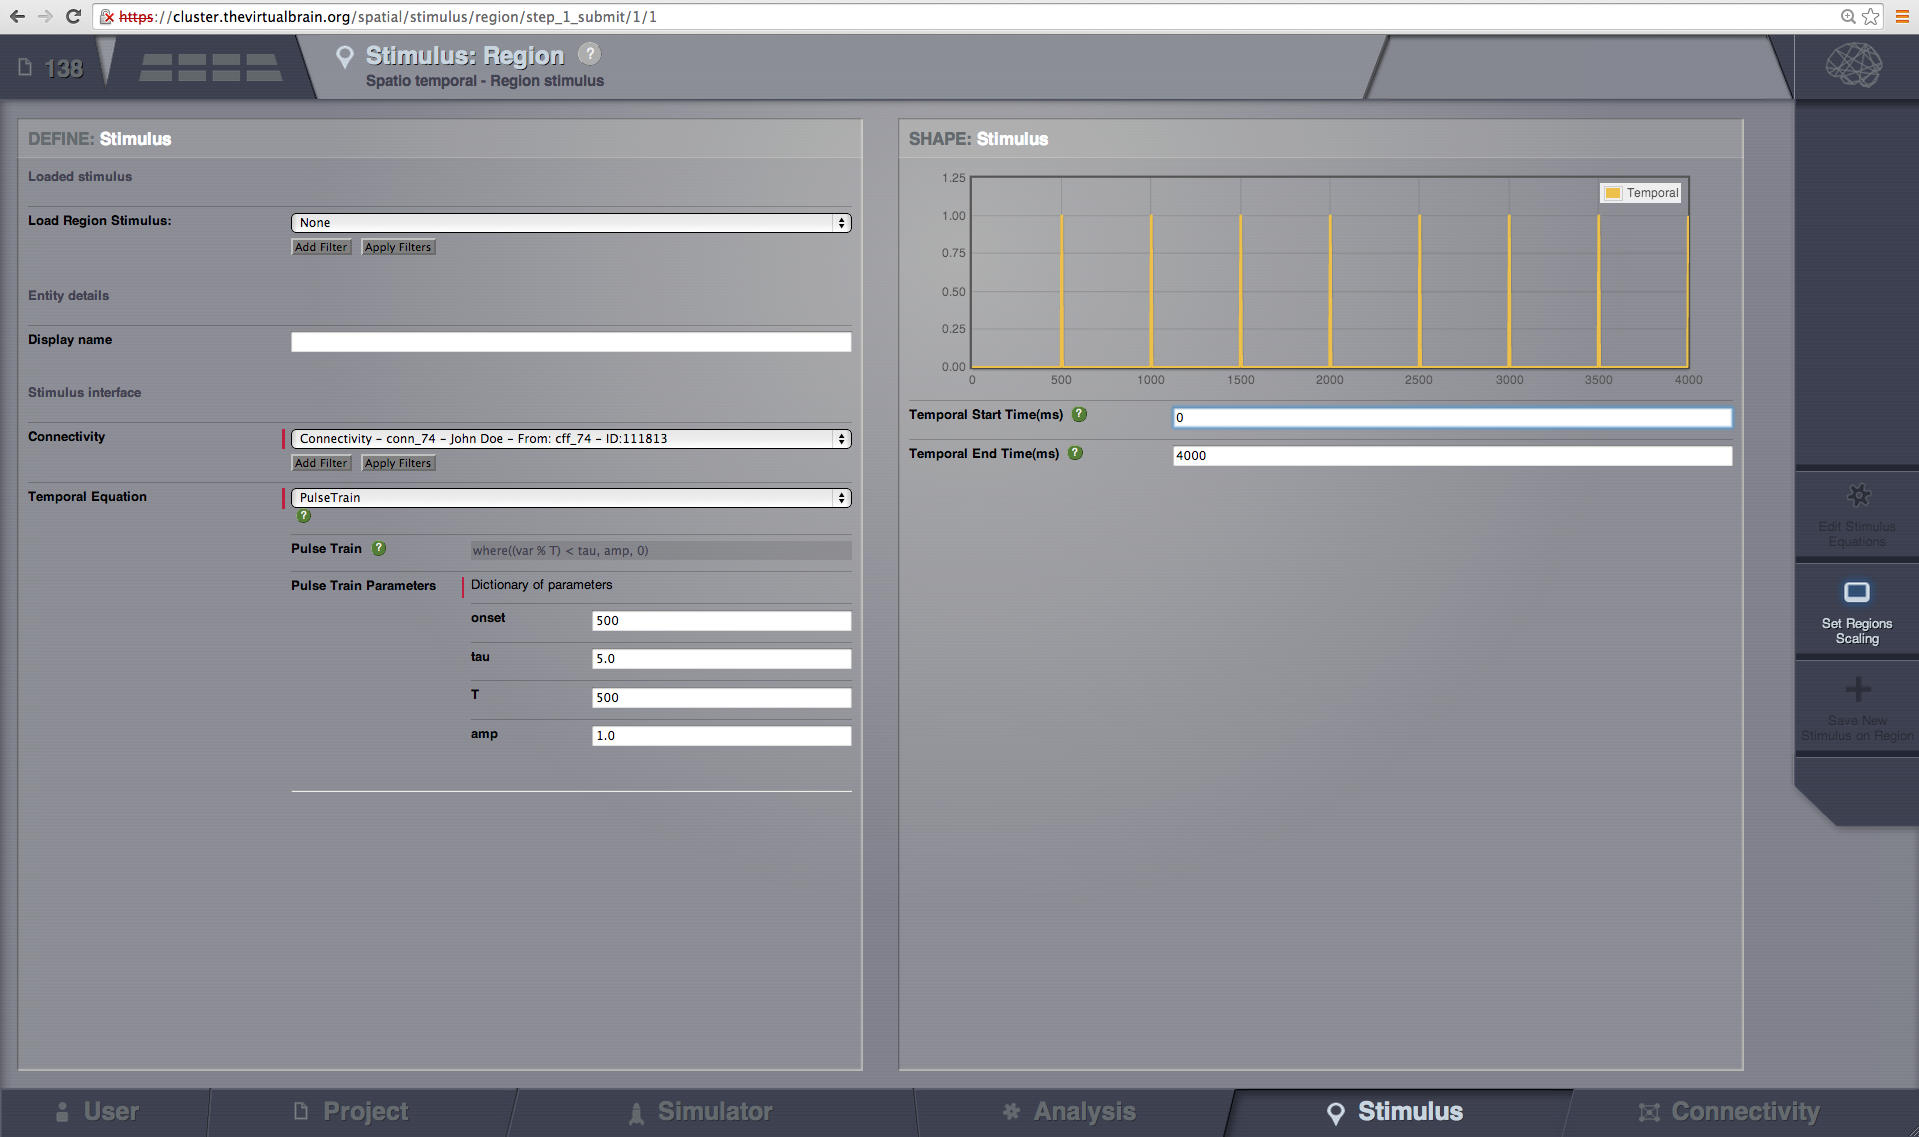
\includegraphics[width=\linewidth]{Handout_UI_HeterogenousModelAndStimulation_StimulusRegion}%
  \caption{Region-based stimulus generation}%
  \label{fig:stimulus_region}%
\end{figure}




\begin{formal}
\begin{enumerate}[resume]
\setcounter{enumi}{3}
\item On the right column you can change the end time to visualize the stimulus. See Fig. \ref{fig:pulse_train}.
\end{enumerate}
\end{formal}

\begin{marginfigure}
  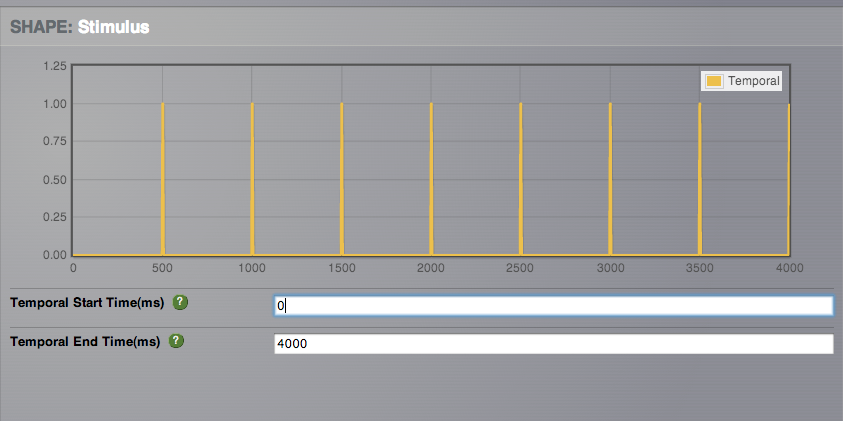
\includegraphics[width=\linewidth]{Handout_UI_HeterogenousModelAndStimulation_PulseTrain}%
  \caption{Square pulse train}%
  \label{fig:pulse_train}%
\end{marginfigure}

 To define which and how much nodes will be affected by a stimulus, a scaling factor per node can be defined. 

\begin{formal}
\begin{enumerate}[resume]
\setcounter{enumi}{4}
\item Click on \underline{Set Region Scalings}. 
\item Unselect all the nodes. Then, select the primary visual cortices, left and right V1, save the selection for later use. (Figs. \ref{fig:unselect_nodes} and \ref{fig:save_selection})
\end{enumerate}
\end{formal}

\begin{figure}[h]
  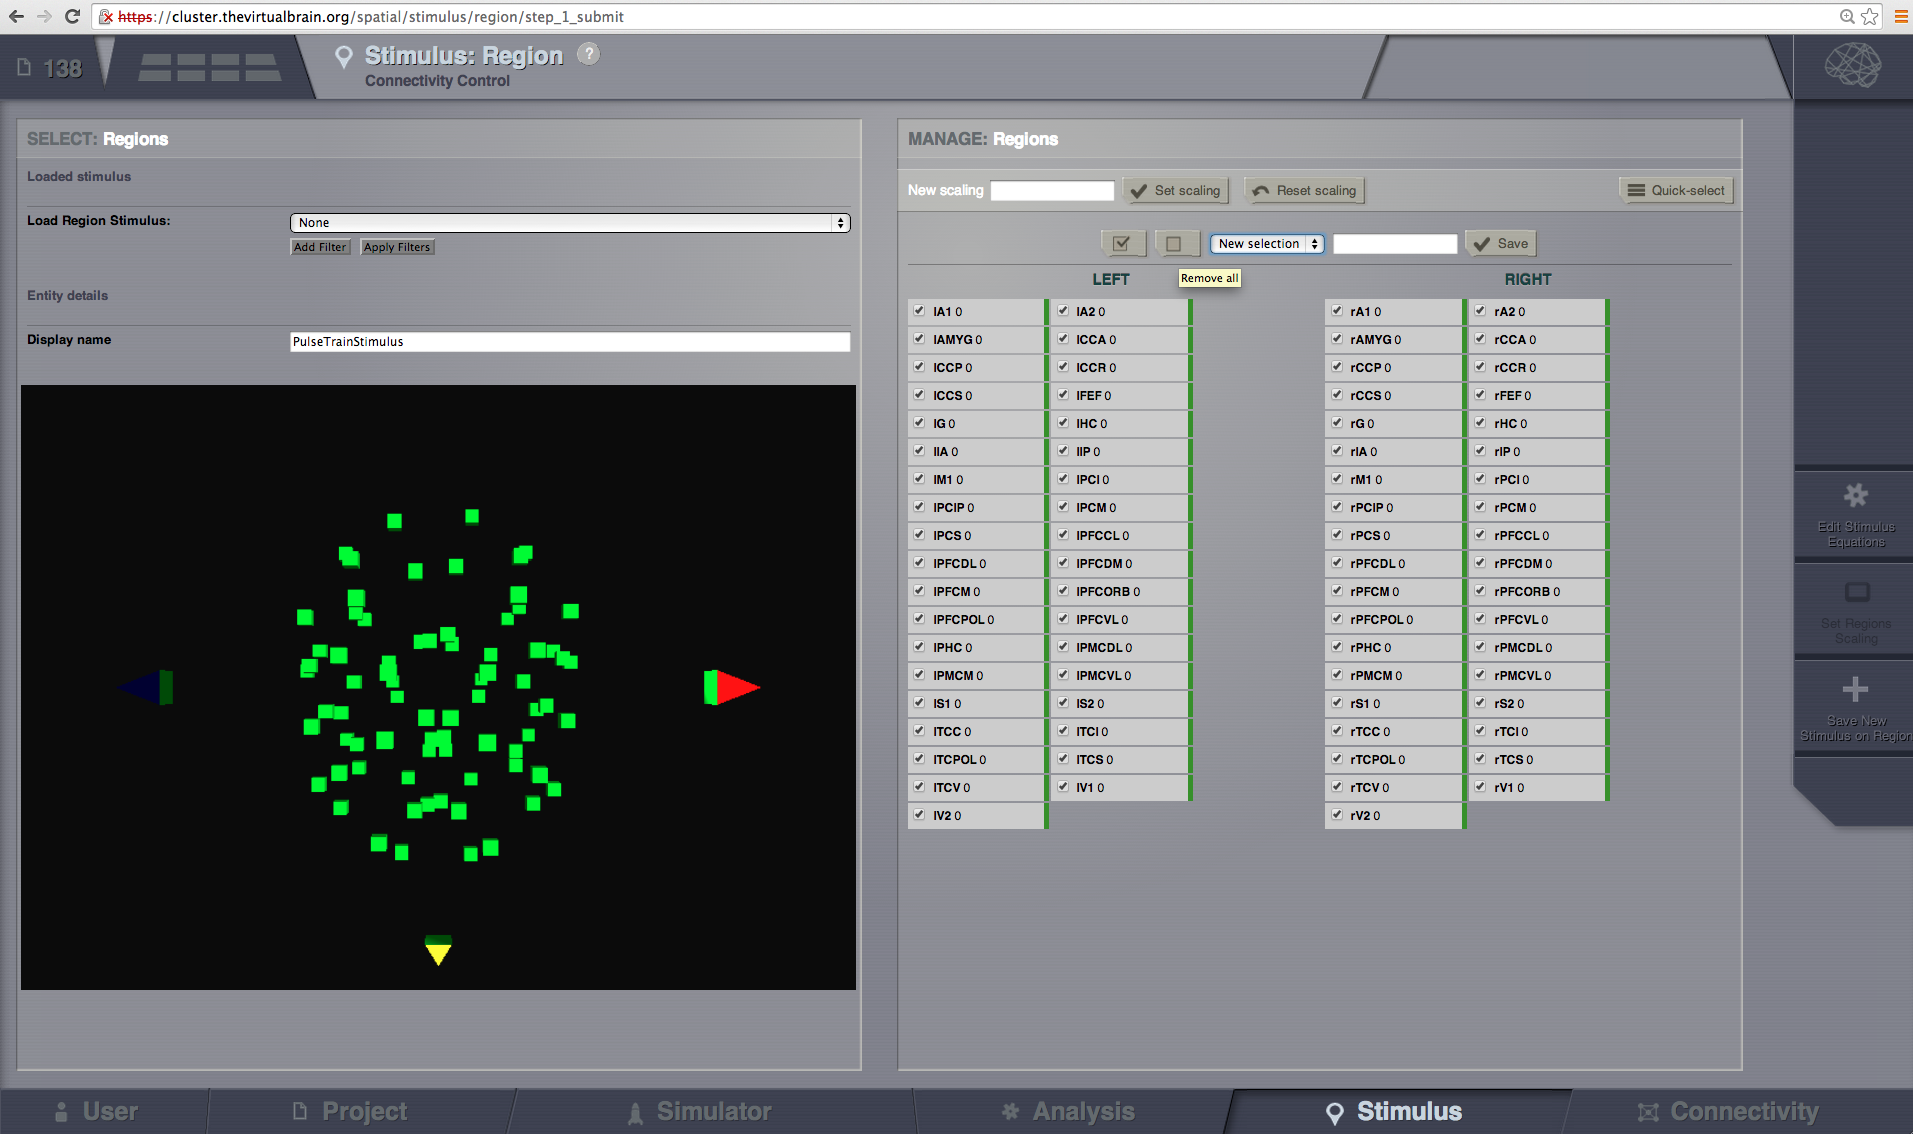
\includegraphics[width=\linewidth]{Handout_UI_HeterogenousModelAndStimulation_StimulusRegionSelectNodes}%
  \caption{Unselect all the nodes}%
  \label{fig:unselect_nodes}%
\end{figure}

\begin{figure}[h]
  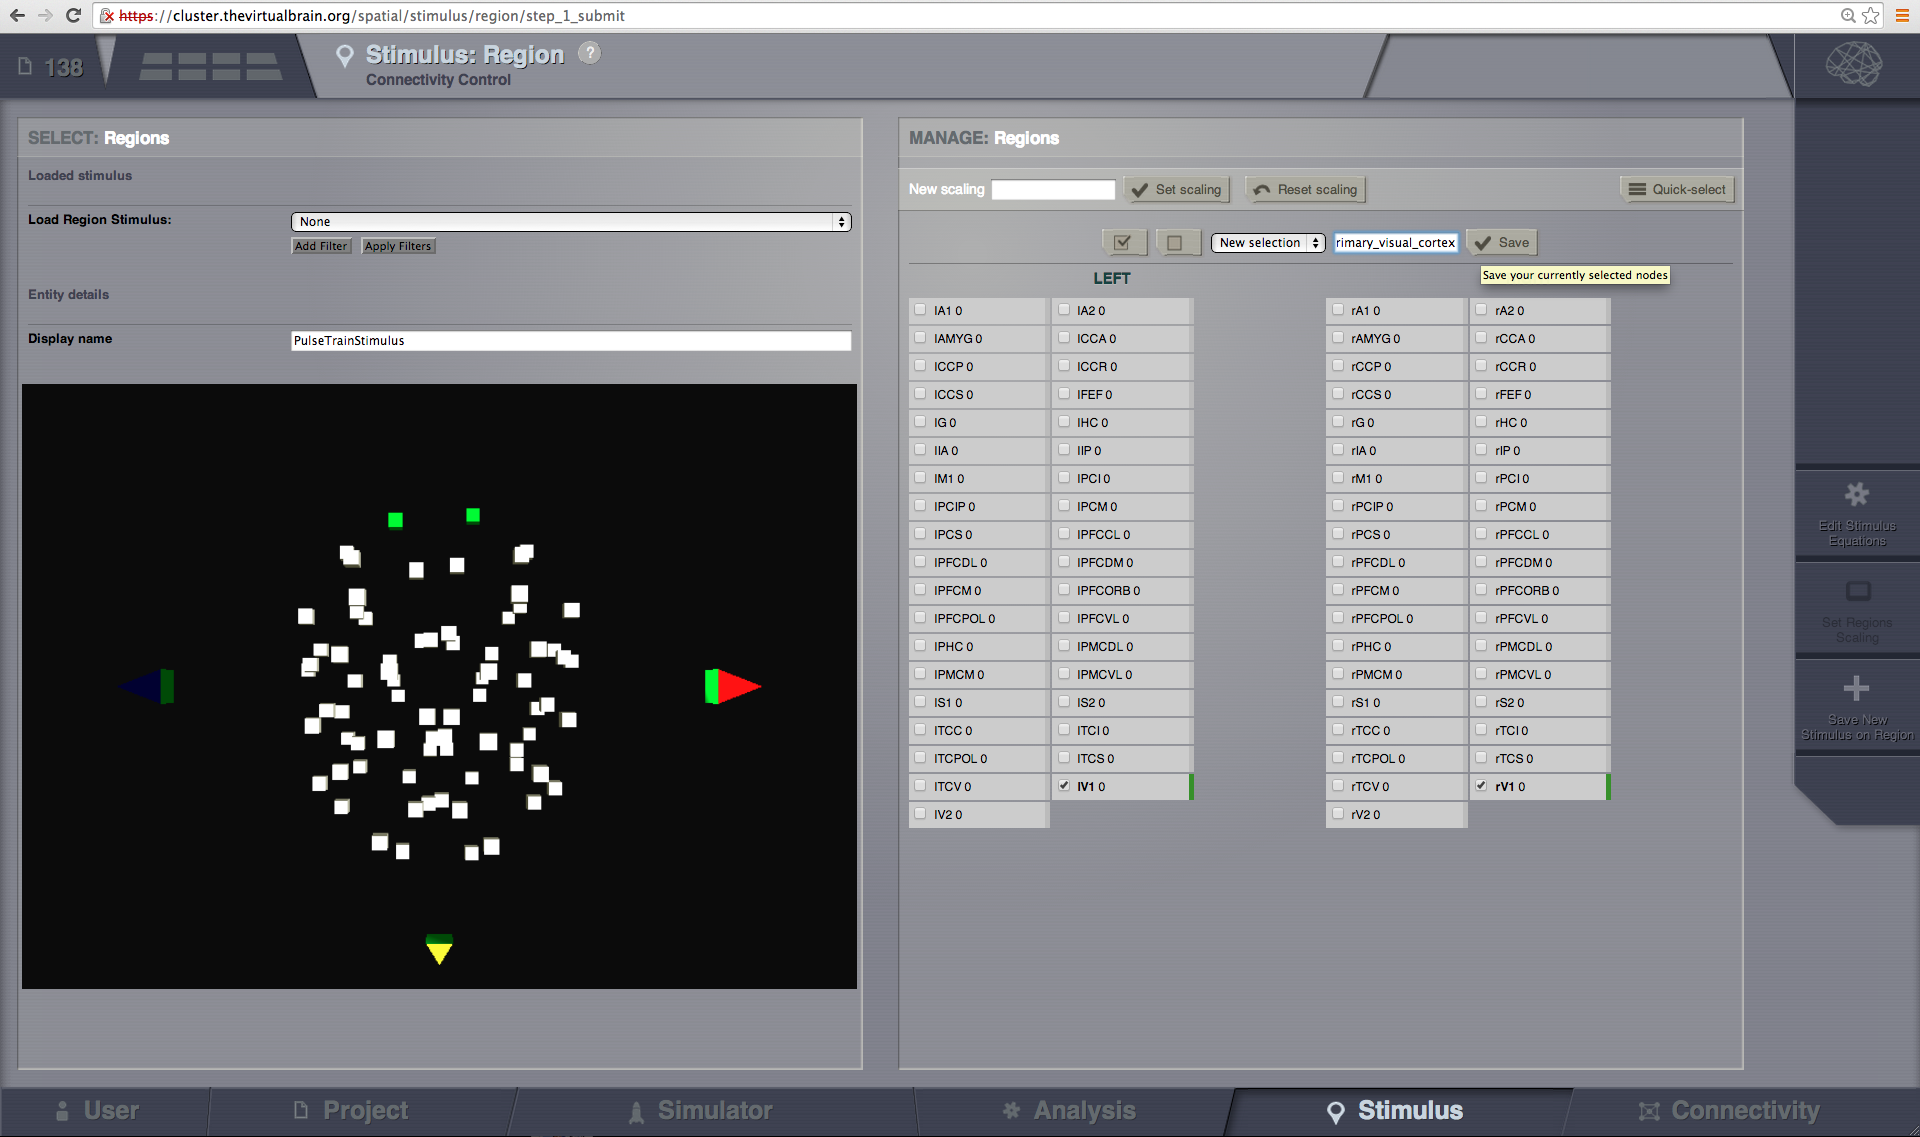
\includegraphics[width=\linewidth]{Handout_UI_HeterogenousModelAndStimulation_StimulusRegionSaveSelection}%
  \caption{Region-based stimulus generation}%
  \label{fig:save_selection}%
\end{figure}

\newpage
\begin{formal}
\begin{enumerate}[resume]
\setcounter{enumi}{6}
\item Set the new scaling to 3.5 -- only those nodes will receive stimulation. 
\item Select all the nodes again and save the stimulus. (Figs. \ref{fig:set_scaling} and \ref{fig:save_scaling} )
\end{enumerate}
\end{formal}

\begin{figure}[h]
  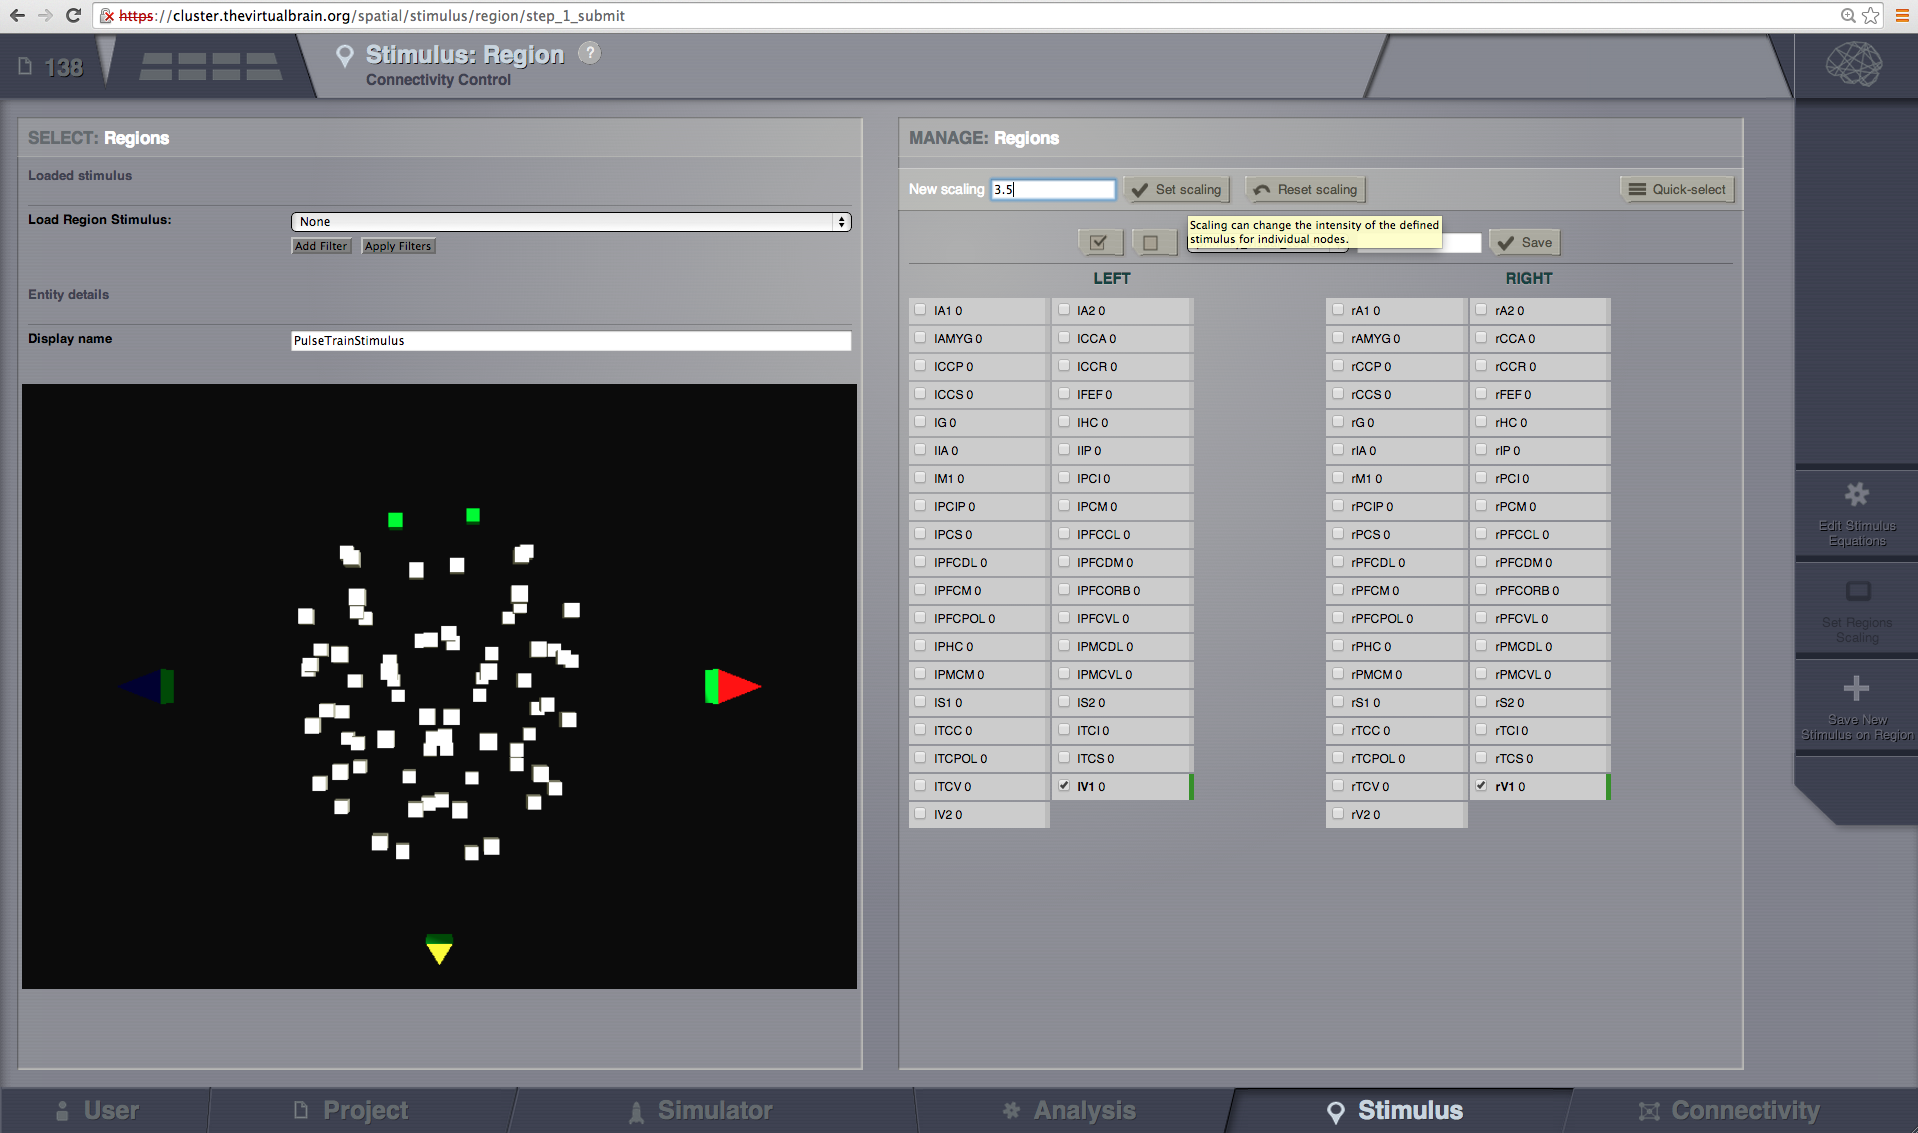
\includegraphics[width=\linewidth]{Handout_UI_HeterogenousModelAndStimulation_StimulusRegionSetScaling}%
  \caption{Unselect all the nodes}%
  \label{fig:set_scaling}%
\end{figure}

\begin{figure}[h]
  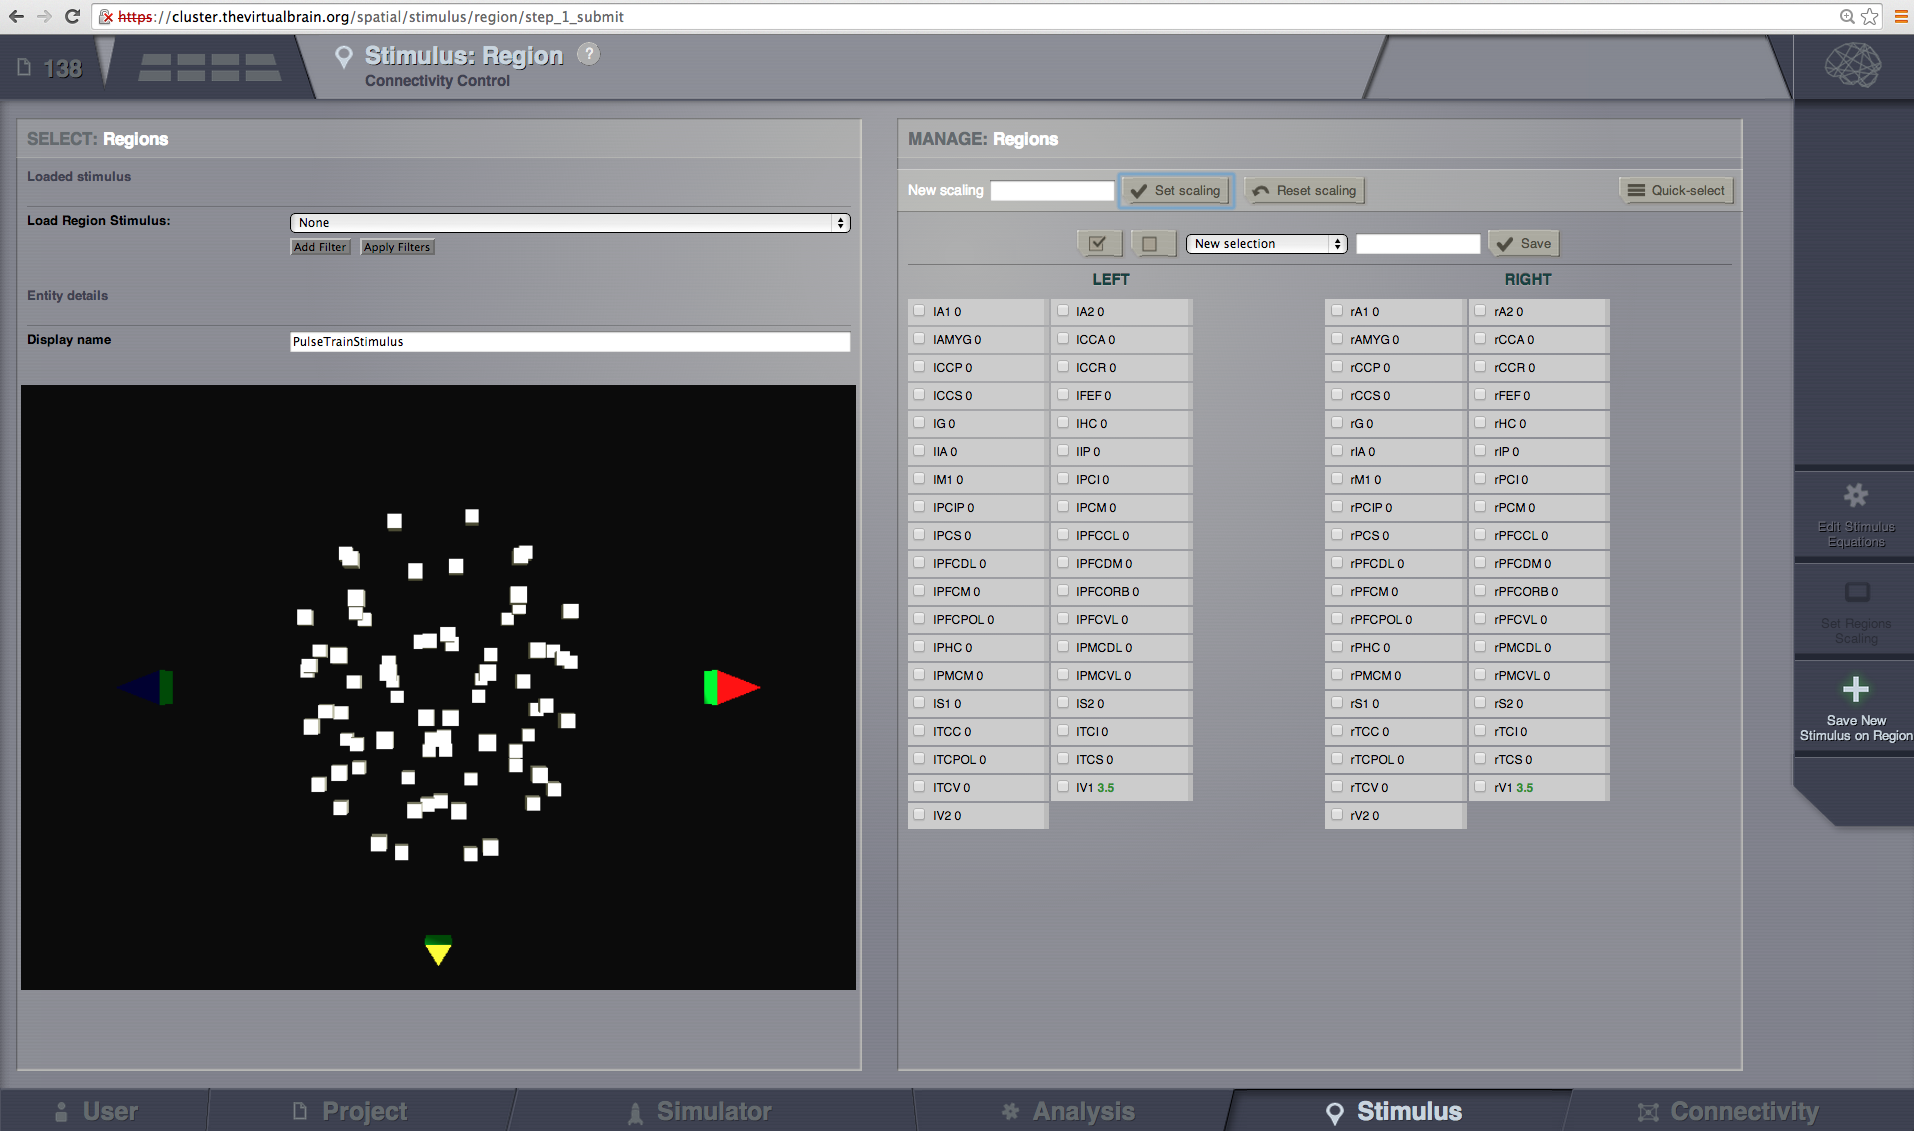
\includegraphics[width=\linewidth]{Handout_UI_HeterogenousModelAndStimulation_StimulusRegionScaling}%
  \caption{Region-based stimulus generation}%
  \label{fig:save_scaling}%
\end{figure}


\newpage
\subsection{Stimuli Generation For Surface-based simulation}\label{sec:surface_stim}

\begin{formal}
\begin{enumerate}
\item Go to \textsc{Stimulus} $\rightarrow$ \textsc{Surface stimulus} area. 
\item As with the region level stimuli, we use an equation to define \underline{the temporal
profile}. The temporal component of the \underline{surface stimulus} will be the same square pulse train as before, except that we'll set the \underline{onset} and the \underline{repetition period} to \textbf{\unit[50]{ms}}.
\item  However, unlike in the region level case, we also use an equation to
define the \underline{spatial profile of the stimulus}. For the spatial profile we'll use e \underline{Sigmoid function} with the only change being the width of the kernel, \underline{sigma}, that we set to \textbf{\unit[10]{mm}}.  Here, as with the \underline{local connectivity}, we
must use an equation which drops toward zero with increasing distance.(Fig. \ref{fig:surface_stimulus})
\end{enumerate}
\end{formal}

\begin{figure}[h]
  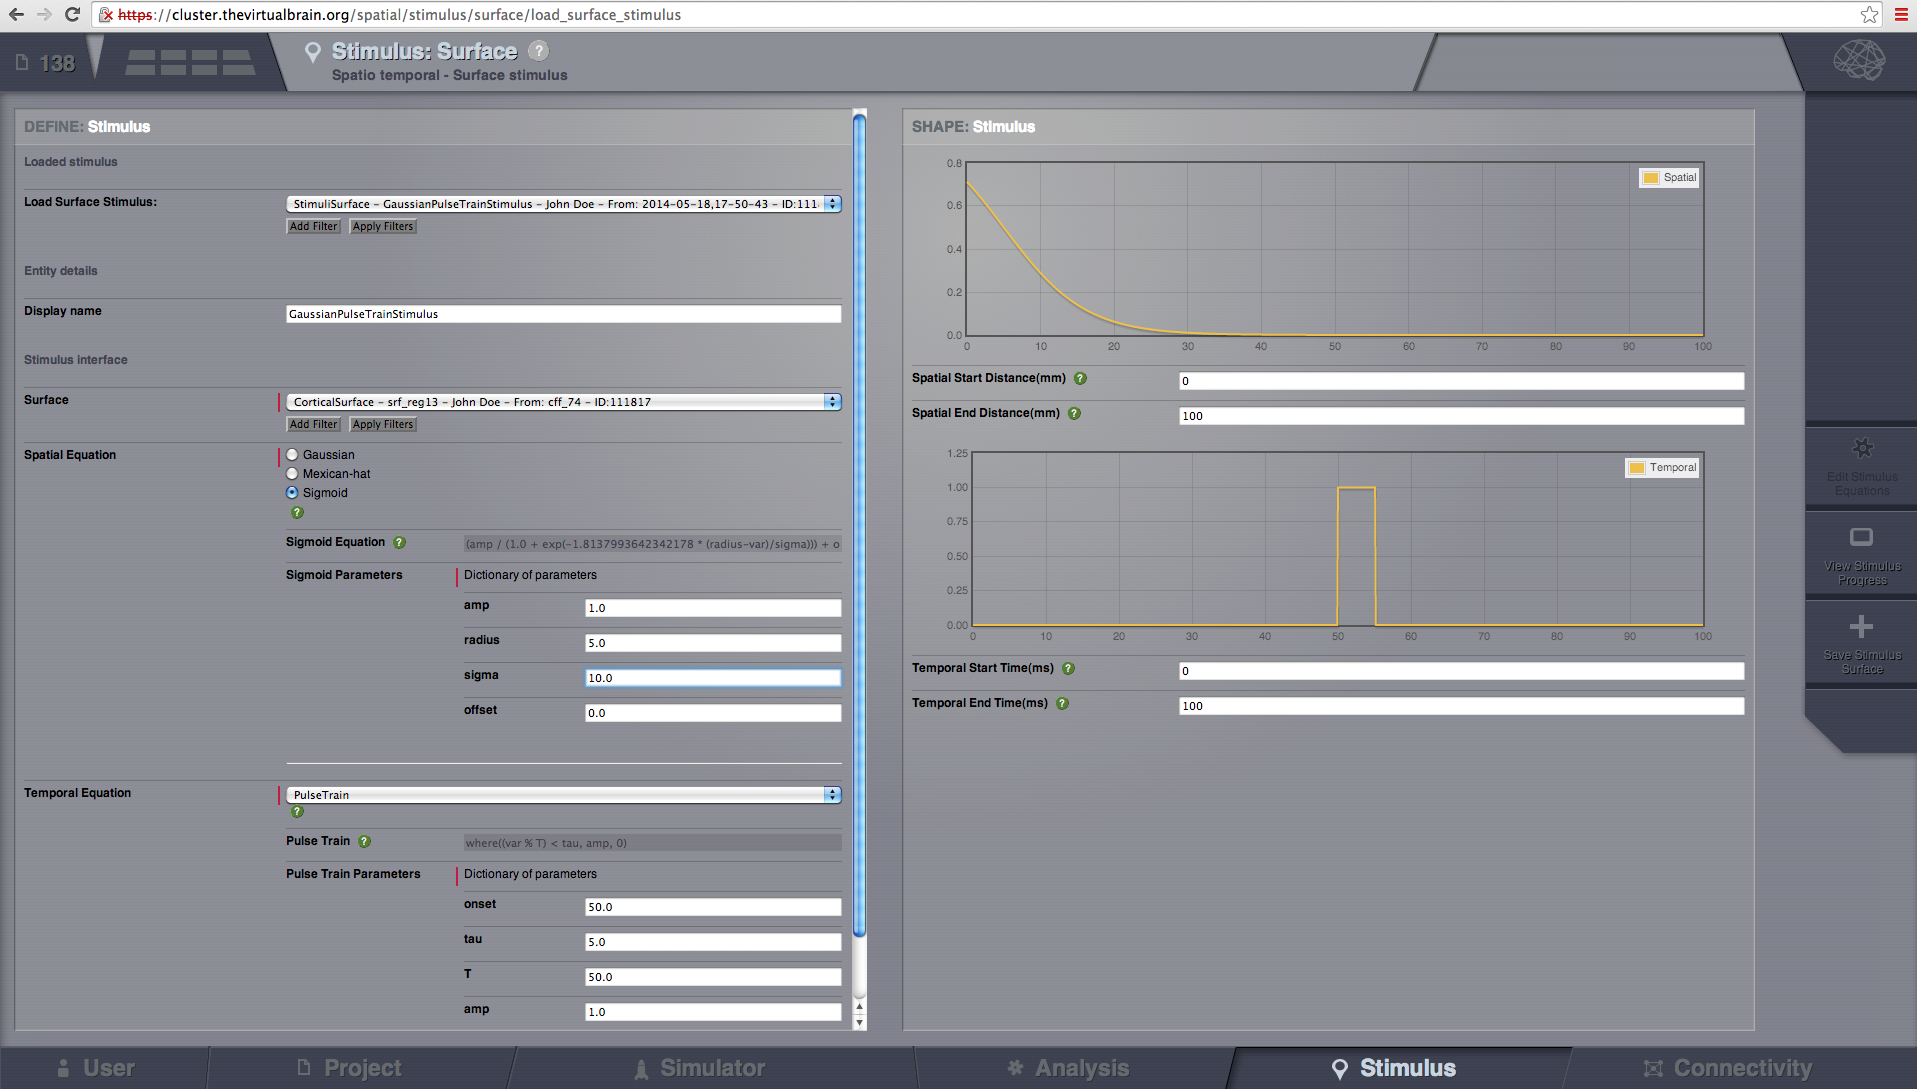
\includegraphics[width=\linewidth]{Handout_UI_HeterogenousModelAndStimulation_StimulusSurface}%
  \caption{Surface-based stimulus generation}%
  \label{fig:surface_stimulus}%
\end{figure}

\begin{formal}
\begin{enumerate}
\setcounter{enumi}{3}
\item We also need to specify one or
more \underline{focal points} (vertices on the cortical surface), about which the
\underline{spatial equation} will be evaluated. To do this we go to \underline{View Stimulus progress} where we can select a few focal points by clicking on the \underline{cortical surface} and then on the \underline{Add focal point} button. (Fig. \ref{fig:focal_points})
\end{enumerate}
\end{formal}

\begin{figure}[h]
  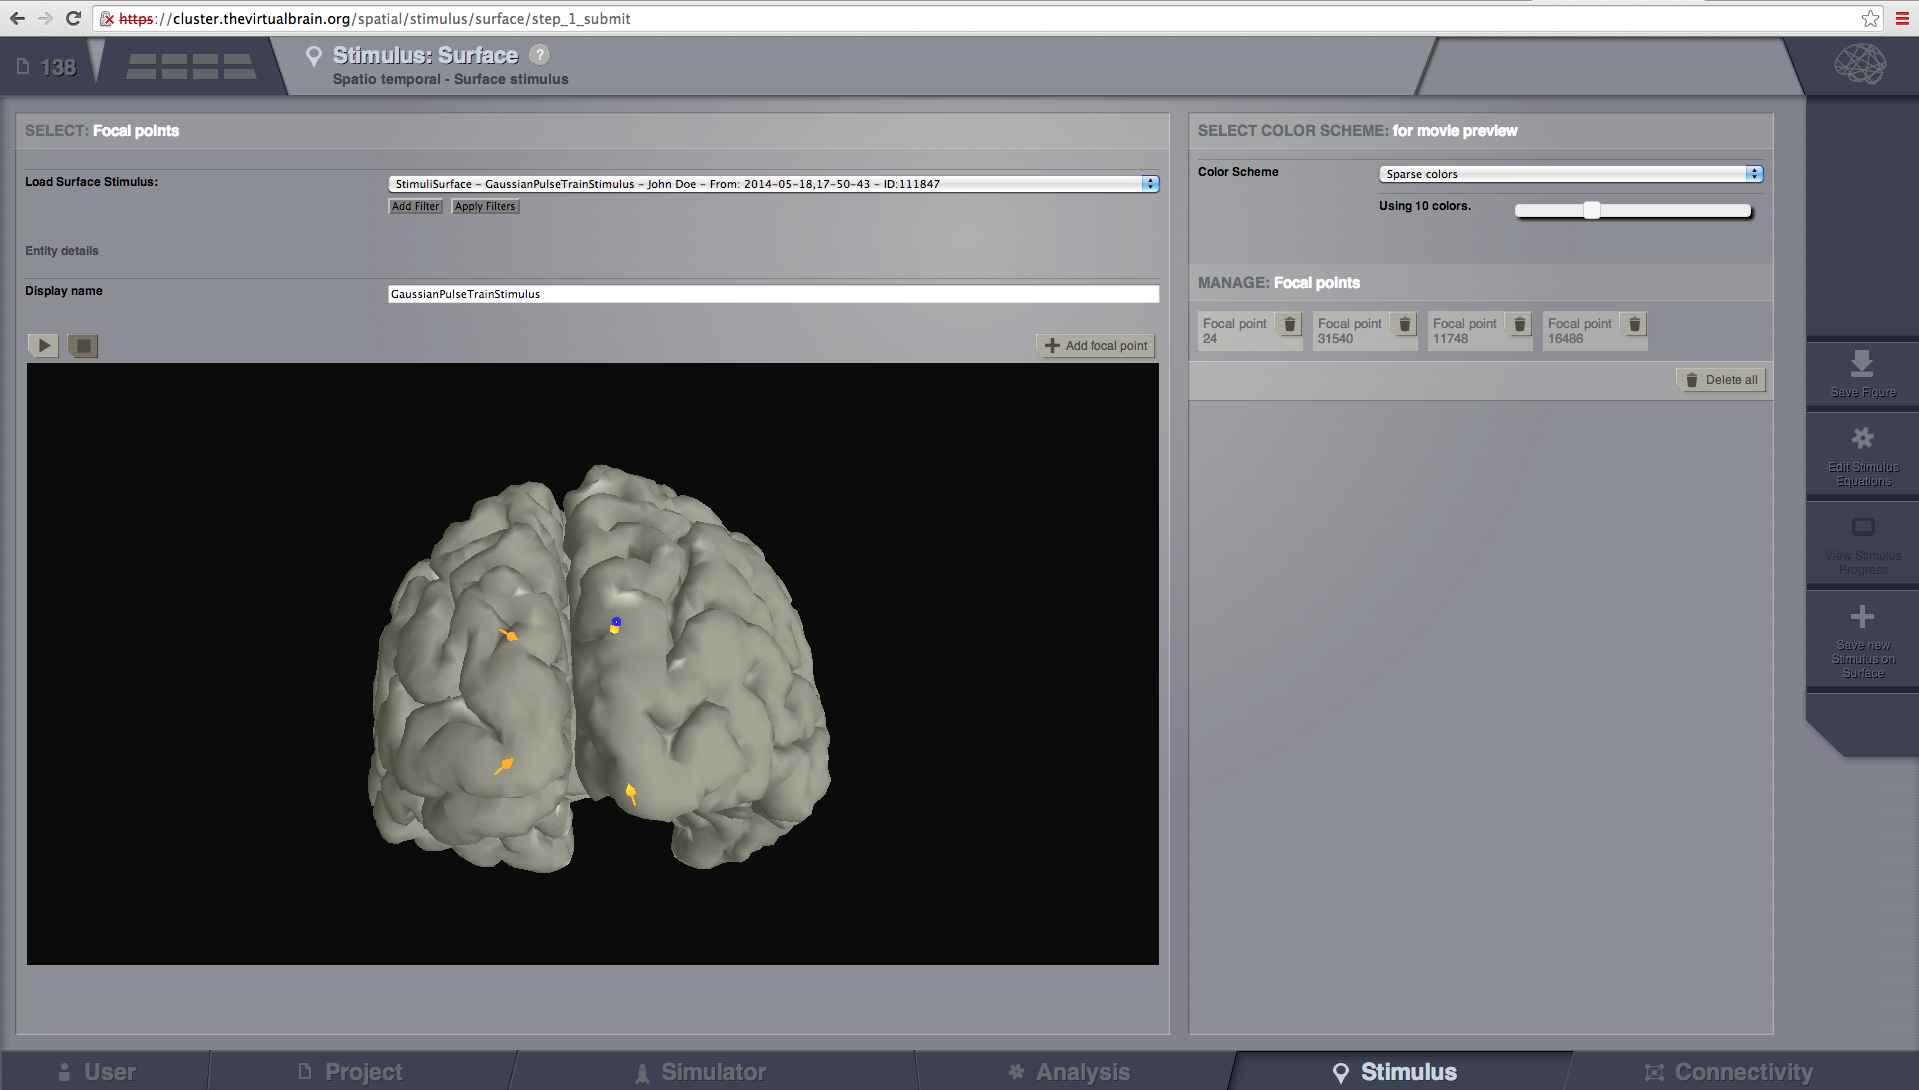
\includegraphics[width=\linewidth]{Handout_UI_HeterogenousModelAndStimulation_StimulusSurfaceFocalPoints}%
  \caption{Add focal points}%
  \label{fig:focal_points}%
\end{figure}

\begin{formal}
\begin{enumerate}
\setcounter{enumi}{4}
\item We save the stimulus and then we can visualize it as a movie. This was already done for you, so you can directly click on 
\includegraphics[width=0.01\textwidth]{butt_launch_project.png}. (Fig. \ref{fig:surface_stim_movie}).
\end{enumerate}
\end{formal}
 
 \begin{marginfigure}
  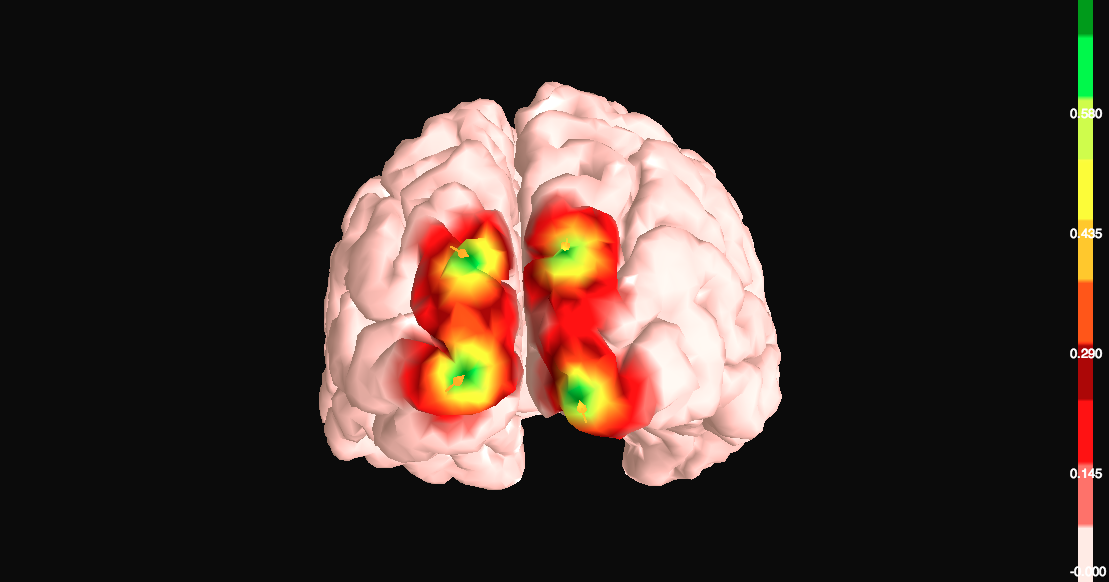
\includegraphics[width=\linewidth]{Handout_UI_HeterogenousModelAndStimulation_StimulusSurfaceMovie}%
  \caption{Have a look at the spatiotemporal profile of the stimulus.}%
  \label{fig:surface_stim_movie}%
\end{marginfigure}


\subsection{Stimulus-driven simulations}\label{sec:stim_sim}

Next, we go back to the \textsc{Simulator} area, and we'll set up the local dynamics using the \underline{generic 2D oscillator.}
\begin{margintable}
  \centering
  \fontfamily{ppl}\selectfont
  \begin{tabular}{ll}
    \toprule
    Model parameter & Value \\
    \midrule
             $a$          &   -0.5   \\
             $b$          &  -15    \\
             $c$           &   0        \\
             $d$           &   0.02    \\
             $e$           &   3        \\
             $f$            &   1    \\
             $g$           &   0        \\
             $I$            &   0        \\
             $\alpha$   &   1        \\
             $\beta$     &   1     \\
             $\gamma$&   1       \\
             $\tau$       &   1 \\
    \bottomrule
  \end{tabular}
  \caption{In this configuration the topology of the phase portrait features a stable fixed point (a stable spiral) with a characteristic frequency of approximately \unit[10]{Hz}. }
  \label{tab:modeltab}
\end{margintable}
\begin{marginfigure}
  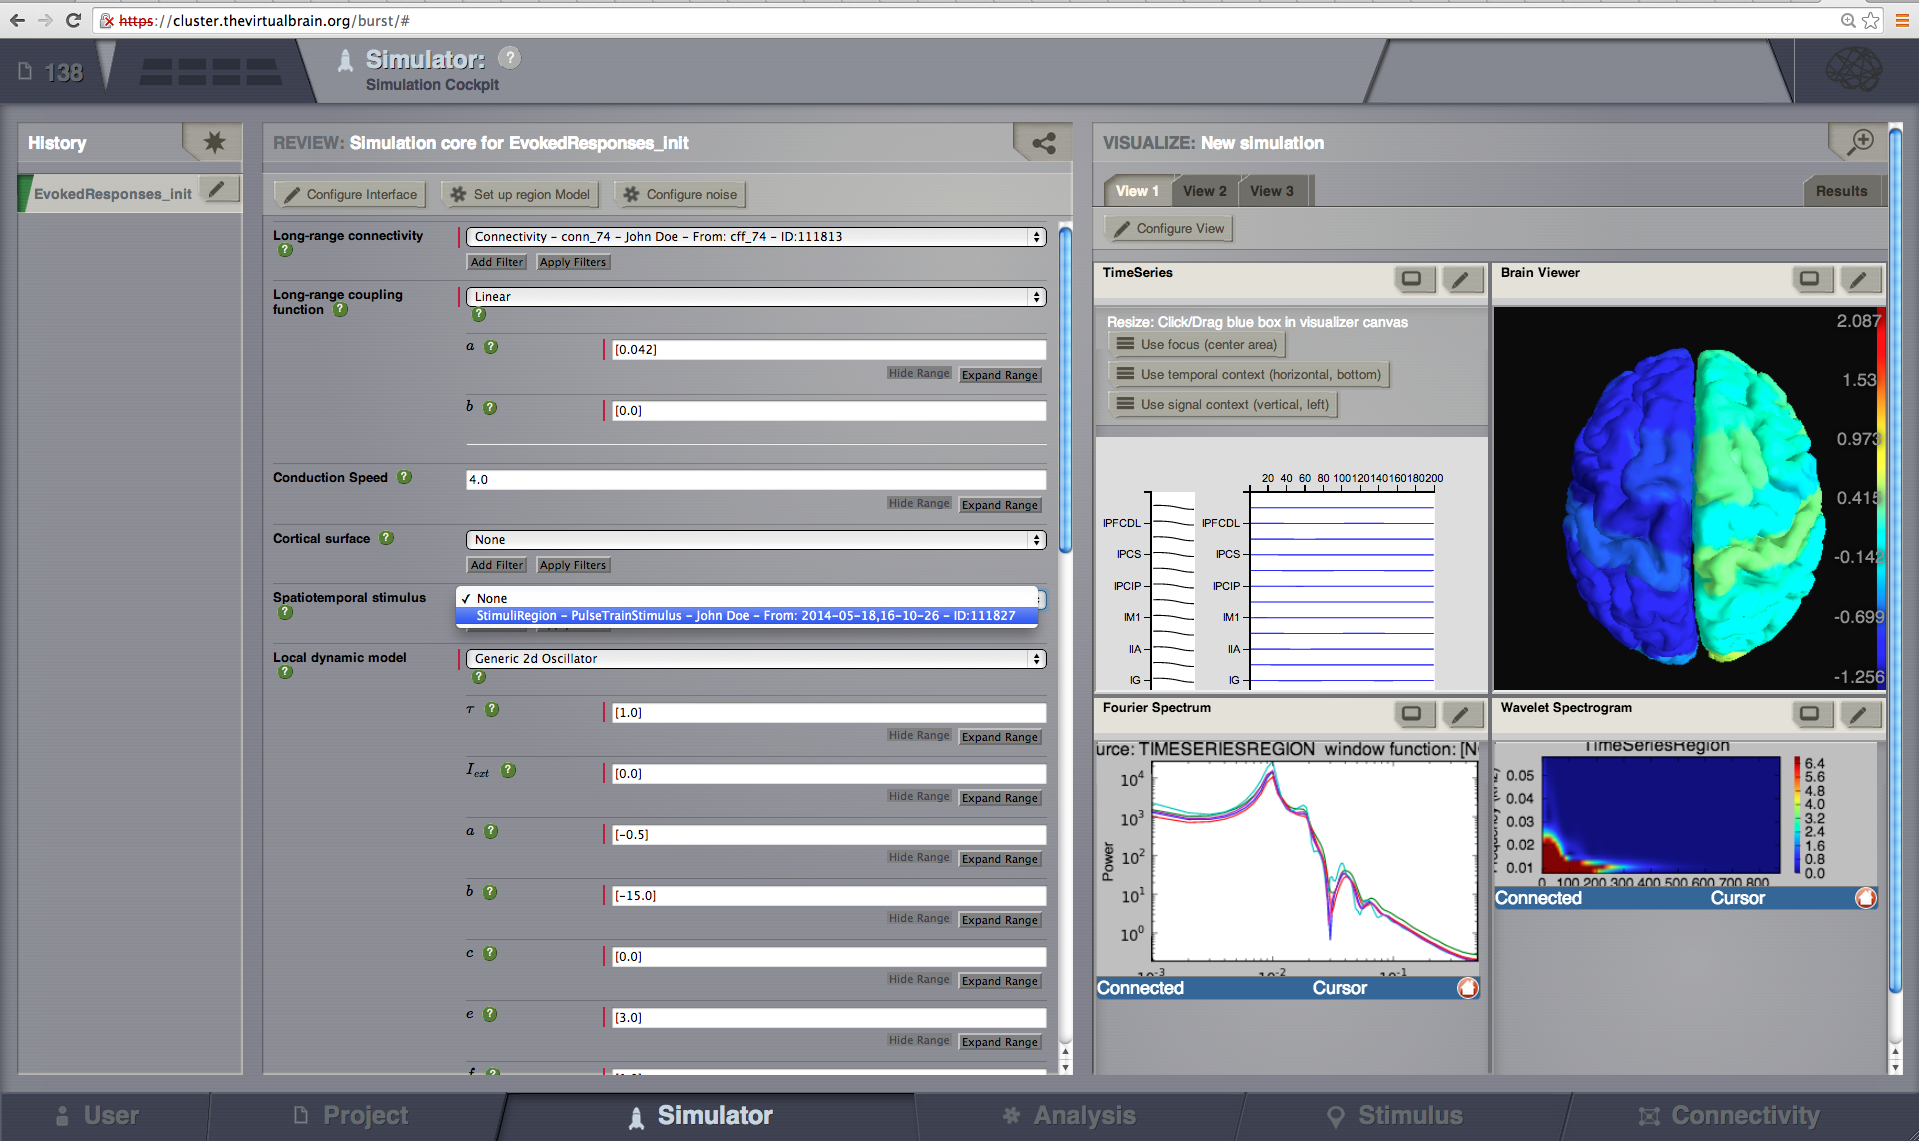
\includegraphics[width=\linewidth]{Handout_UI_HeterogenousModelAndStimulation_RegionAddStimulus}%
  \caption{Add a stimulation pattern}%
  \label{fig:add_stimulus}%
\end{marginfigure}
\begin{simulation}
\begin{enumerate}
\item Now we'll build the model using the \underline{Connectivity}, \underline{Model}, \underline{Integrator} and \underline{Monitors} as in \citep{Sanz-Leon_2013}. You can check the local dynamics using the phase plane interactive tool. The model parameters are specified in Table \ref{tab:modeltab}.
\item Remember the branching mechanism? Before applying the stimulus to our model we'll let the system reach a steady state first, to avoid the intial transient to mask the effect of the stimulation. This is what you have in \textit{EvokedResponses\_init}
\item Run a simulation for \textbf{\unit[1000]{ms}}, with \underline{HeunDeterministic} and $\mathbf{dt=}$\textbf{\unit[0.1]{ms}}; use the \underline{Temporal Average} monitor with a \underline{sample period} equal to \textbf{\unit[1]{ms}}
\item Next, we add a stimulation pattern  (Fig. \ref{fig:add_stimulus}) and continue the simulation for another \textbf{\unit[4000]{ms}}.
\end{enumerate}
\end{simulation}




 Results are in \textit{EvokedResponses\_init} and  \textit{EvokedResponses\_init\_branch1}.

\begin{simulation}
\begin{enumerate}[resume]
\setcounter{enumi}{4}
\item Finally, repeat steps 1-4 using a stochastic integration: \underline{HeunStochastic}; \underline{additive noise} with $\mathbf{D}=$\textbf{\unit[0.005]{au}} and $\mathbf{dt=}$\textbf{\unit[0.1]{ms}}.
These are the simulations in \textit{EvokedResponses\_init\_stochastic} and \textit{EvokedResponses\_init\_stochastic\_branch1}.
\end{enumerate}
\end{simulation}


\newpage

Now, we'll have a look at the resulting time-series.
\begin{marginfigure}
  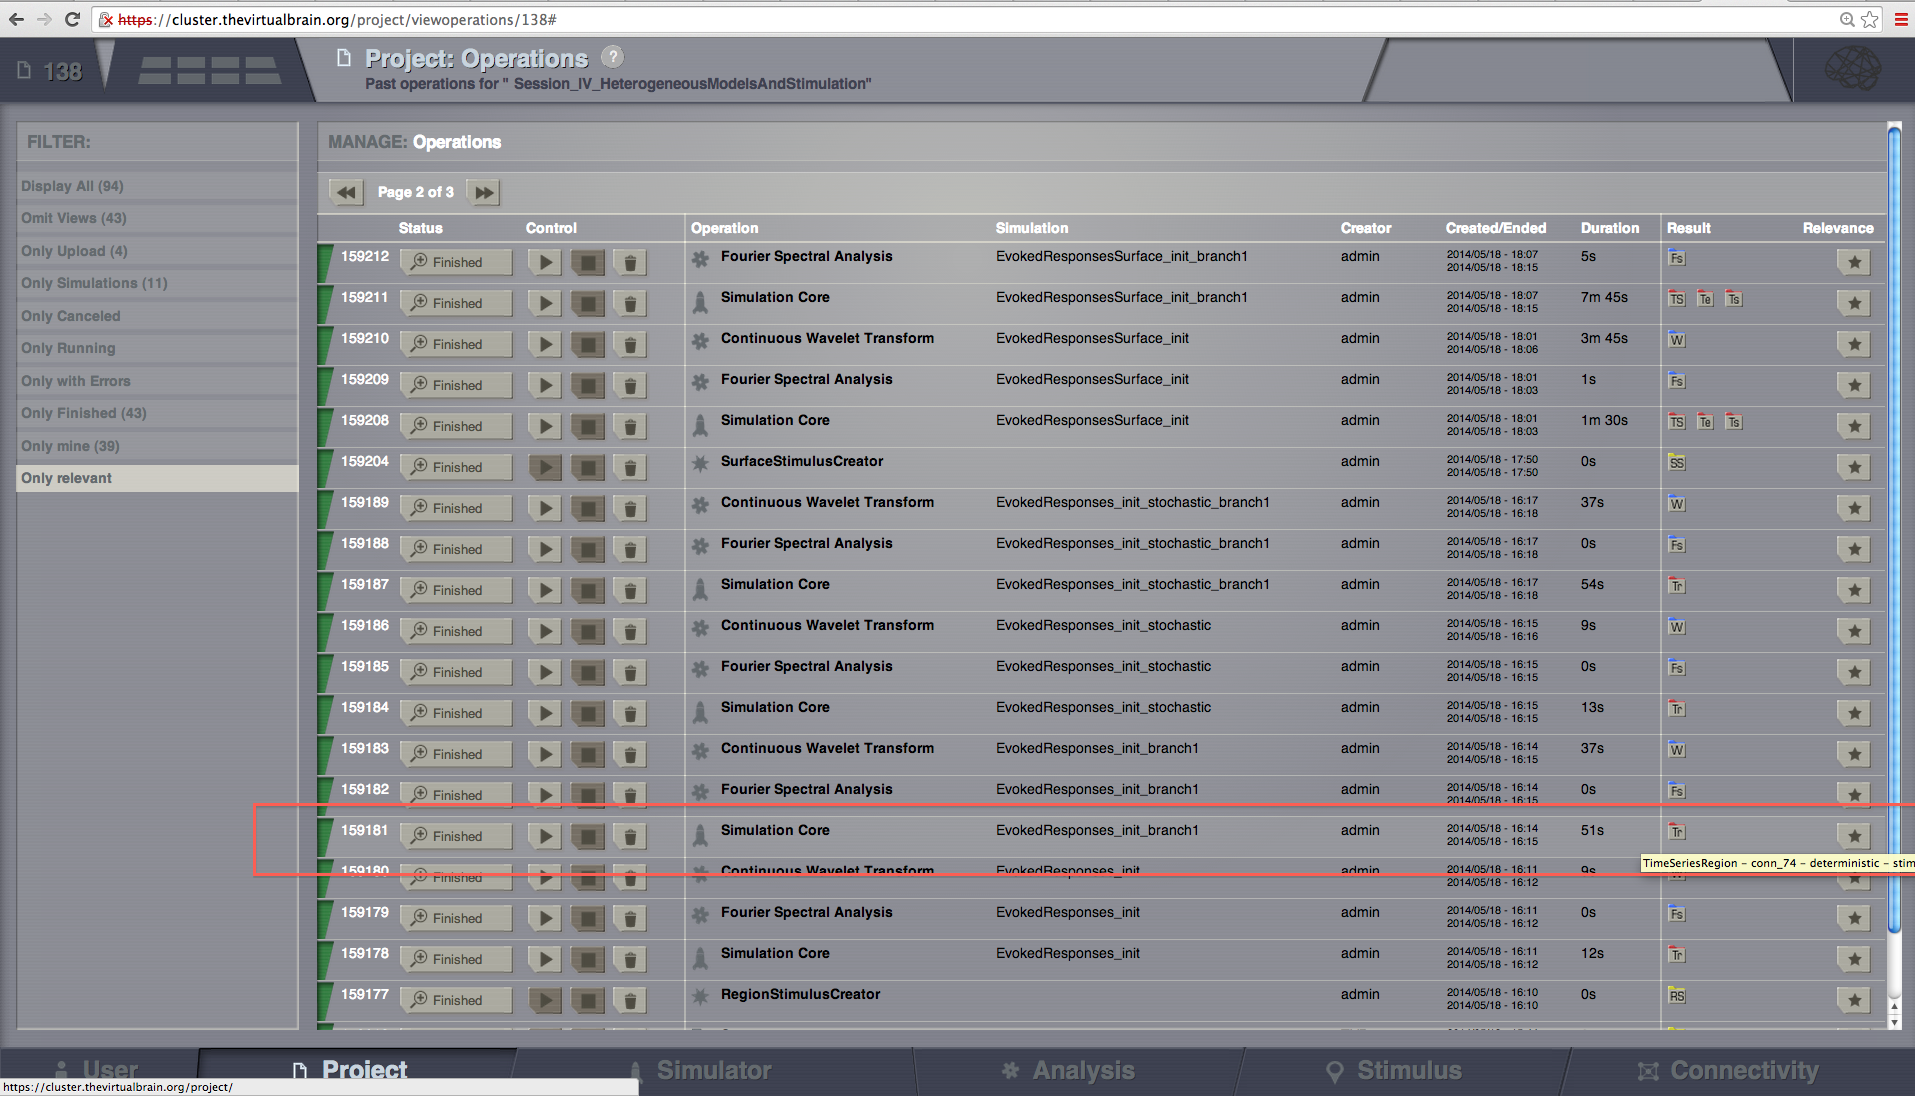
\includegraphics[width=\linewidth]{Handout_UI_HeterogenousModelAndStimulation_OperationDashboard}%
  \caption{Select a time-series}%
  \label{fig:operation_dashboard}%
\end{marginfigure}
\begin{marginfigure}
  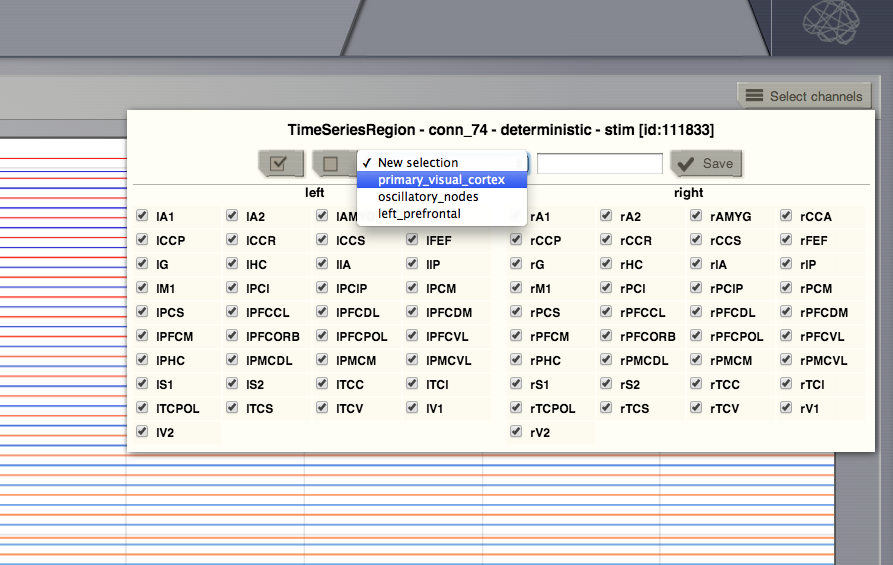
\includegraphics[width=\linewidth]{Handout_UI_HeterogenousModelAndStimulation_VisualCortex}%
  \caption{Use the node selection \textit{primary\_visual\_cortex}}%
  \label{fig:node_selection}%
\end{marginfigure}

\begin{marginfigure}
  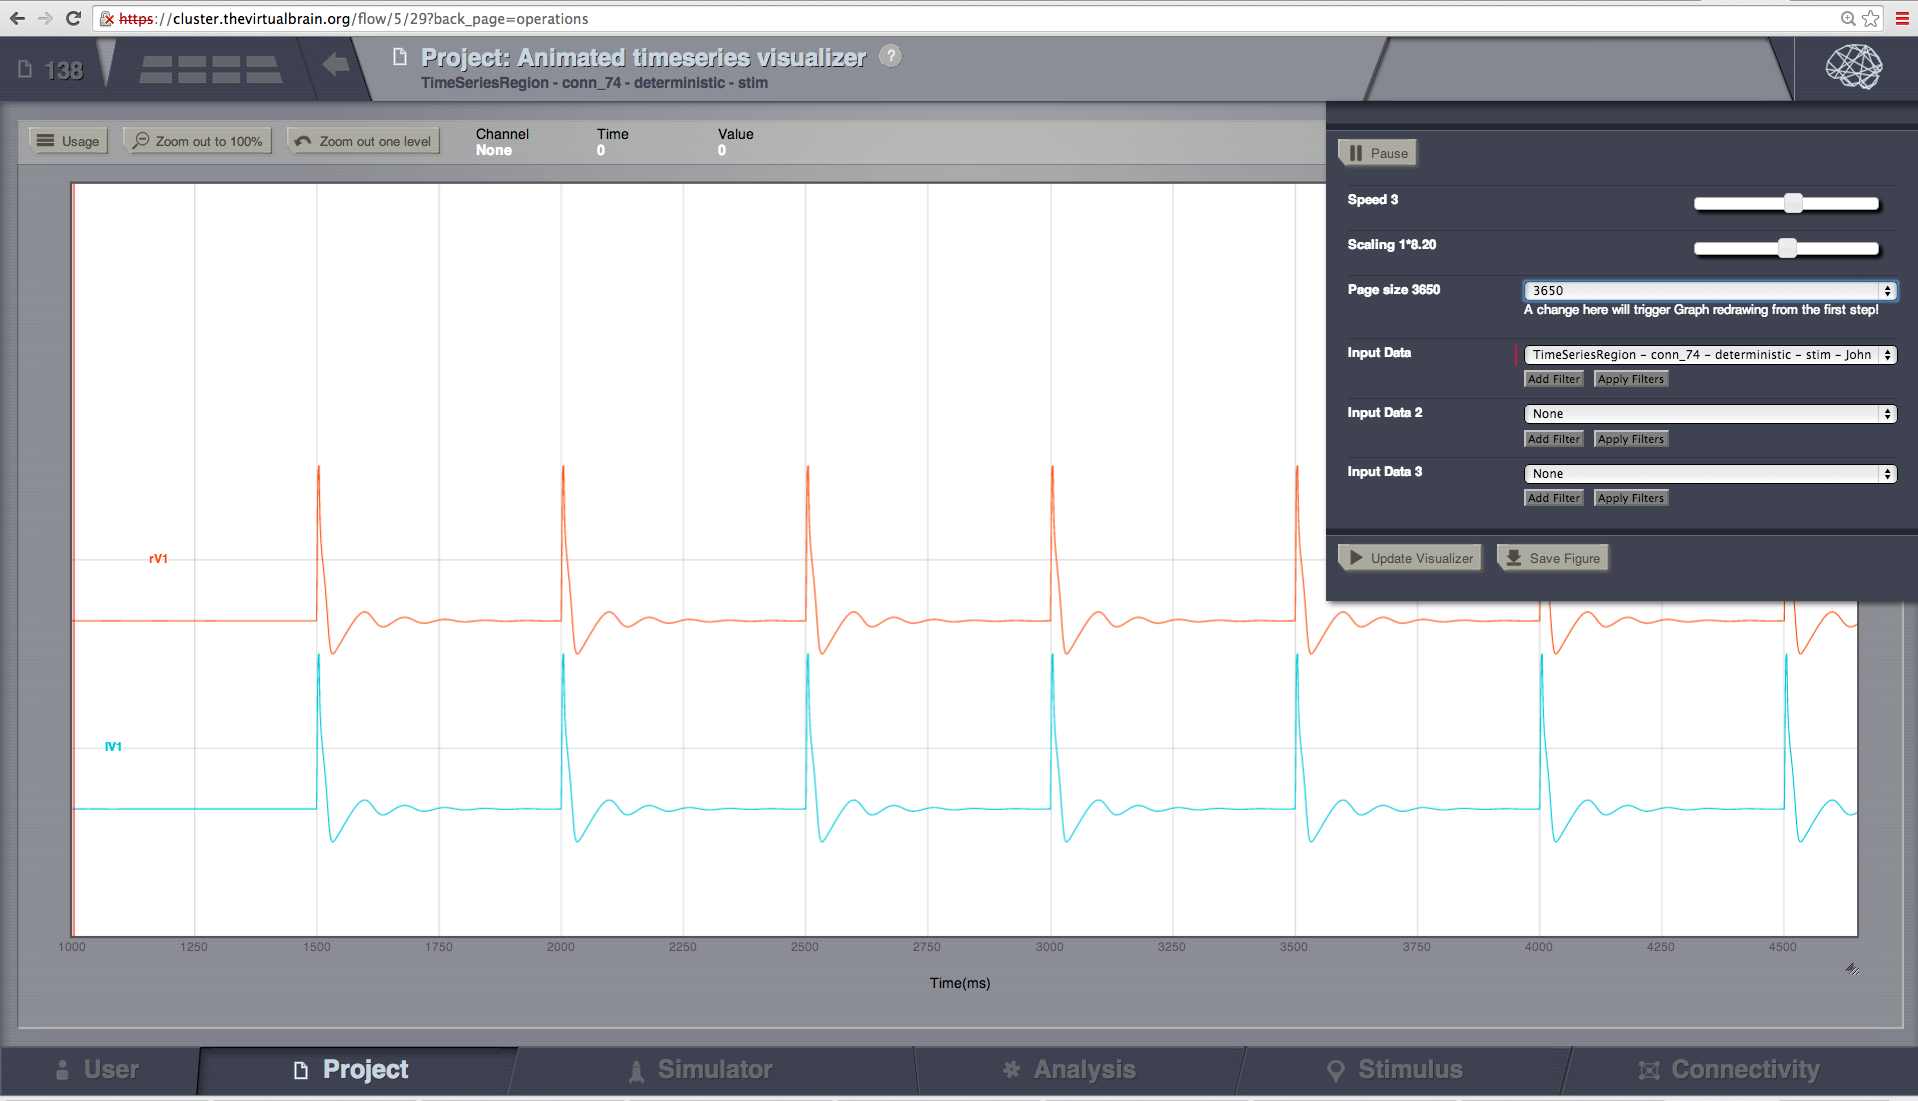
\includegraphics[width=\linewidth]{Handout_UI_HeterogenousModelAndStimulation_AnimatedTimeSeries}%
  \caption{Change the page size}%
  \label{fig:page_size}%
\end{marginfigure}

\begin{marginfigure}
  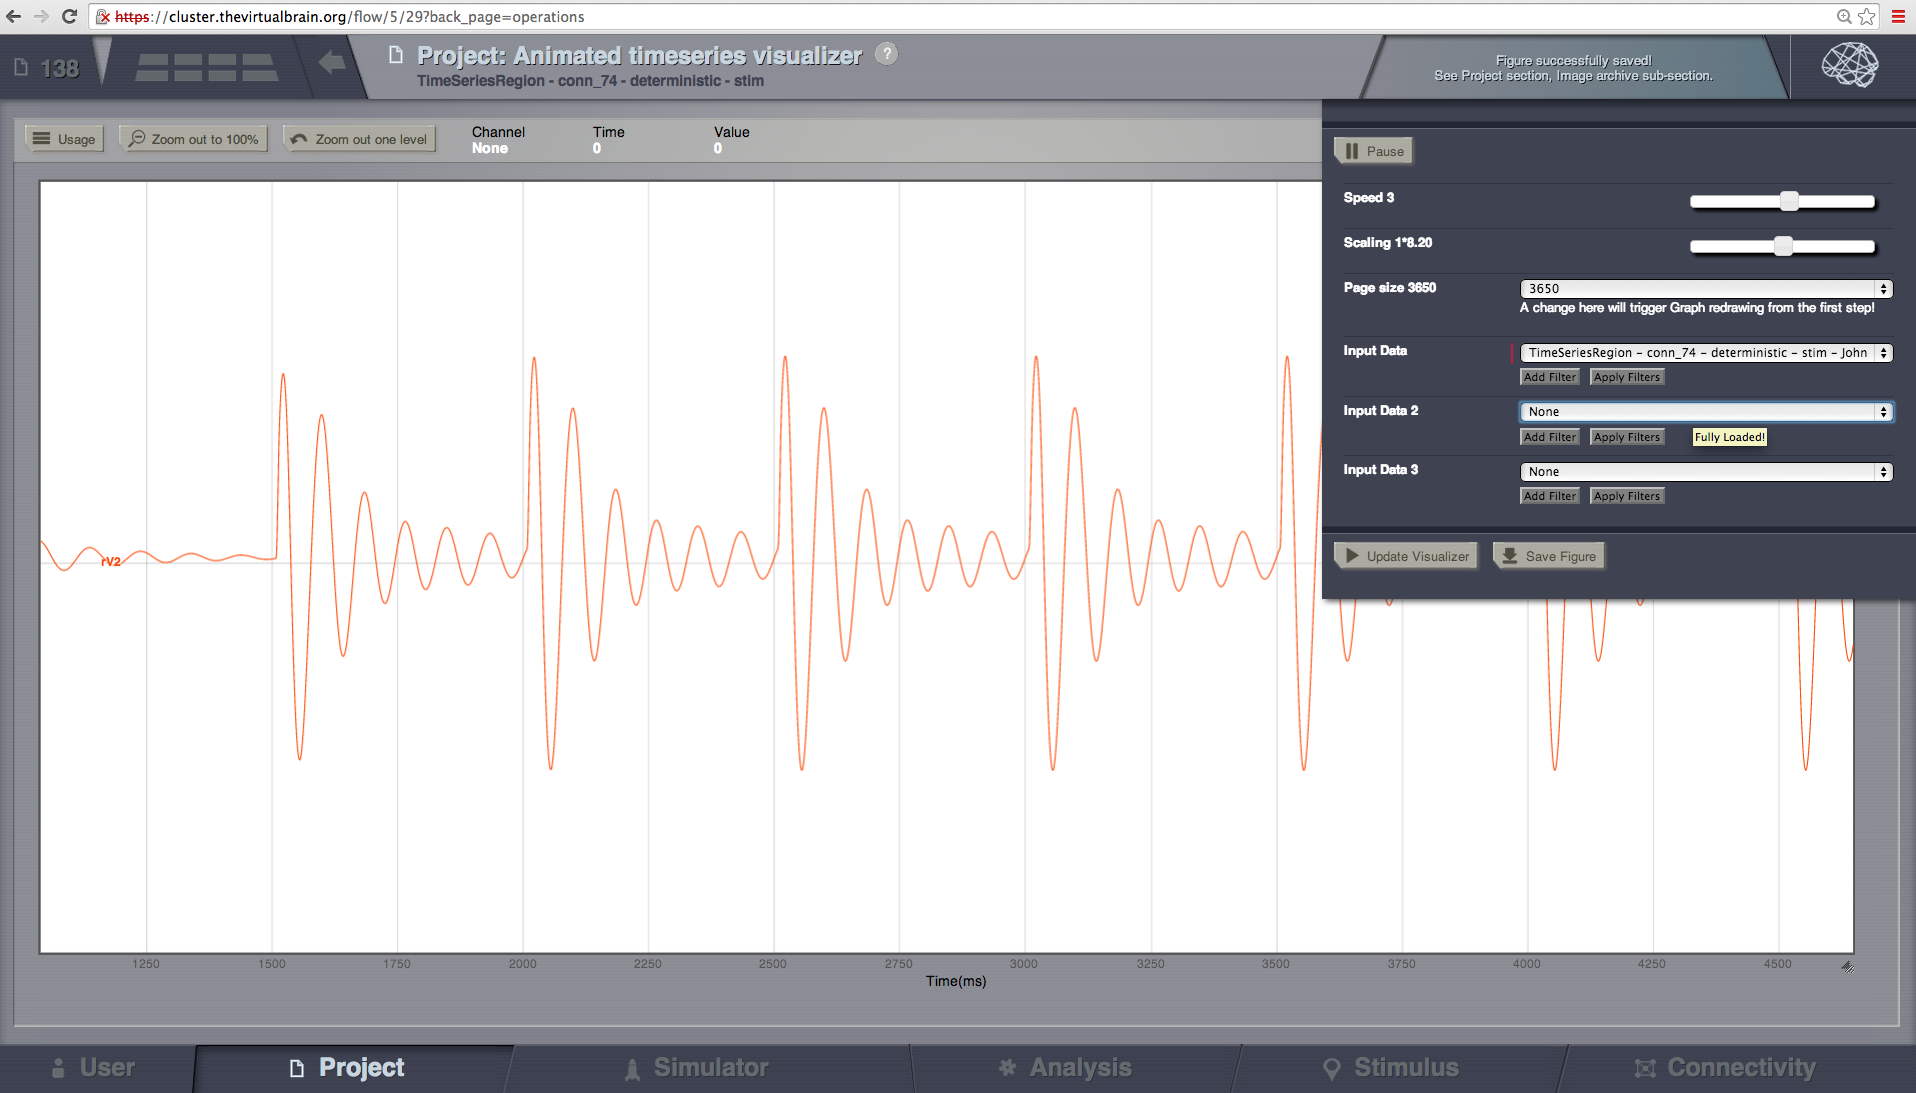
\includegraphics[width=\linewidth]{Handout_UI_HeterogenousModelAndStimulation_ZoomIn}%
  \caption{Left V2: zoom in}%
  \label{fig:zoom_in}%
\end{marginfigure}
\begin{formal}
\begin{enumerate}
\item From the \textsc{Operation dashboard}, select  the time-series  
\includegraphics[width=0.05\textwidth]{nodeTimeSeriesRegion.png} from \textit{EvokedResponses\_init\_branch1}. Then, from the \underline{Visualizer} tab launch the \underline{Animated time series} visualizer. (Fig. \ref{fig:operation_dashboard}).
\item The node selection we saved when we created the stimulus is available. You can directly select the nodes were stimulation was applied. (Fig. \ref{fig:node_selection}). 
You'll have to change the page size, that is how many time points are displayed. (Fig. \ref{fig:page_size}).
\item The stimulus was applied to V1, however if we select left V2 and zoom in we can see the effect of the stimuls. (Fig. \ref{fig:zoom_in})
\end{enumerate}
\end{formal}

\begin{simulation}
\begin{enumerate}
\item For \underline{surface simulations}, select the default \underline{cortical surface} and the \underline{local connectivity}.
\item In addition we set up a few \underline{Monitors}: \underline{EEG, Spatial Average and Temporal Average}.
\item As with the region simulations we'll first run a \underline{short simulation}, \textbf{\unit[200]{ms}} to clear out the initial transient.
\item Add the \underline{Surface stimulus} and continue the simulation for \textbf{\unit[4000]{ms}}. This is a full brain network model making use of all the components of TVB. Results are in \textit{EvokedResponsesSurface\_init} and \textit{EvokedResponsesSurface\_init\_branch1}.
\end{enumerate}
\end{simulation}

 
\begin{blah}
Note that surface simulations can also be run with stimuli defined at the
region level. In this case, all the vertices that belong to one region will
receive the same stimulus. This is what we did in \textit{EvokedResponsesSurface\_init\_branch2}. The differences are shown in Figs. \ref{fig:surfstim_surfsim} and \ref{fig:regstim_surfsim}
\end{blah}

\begin{marginfigure}
  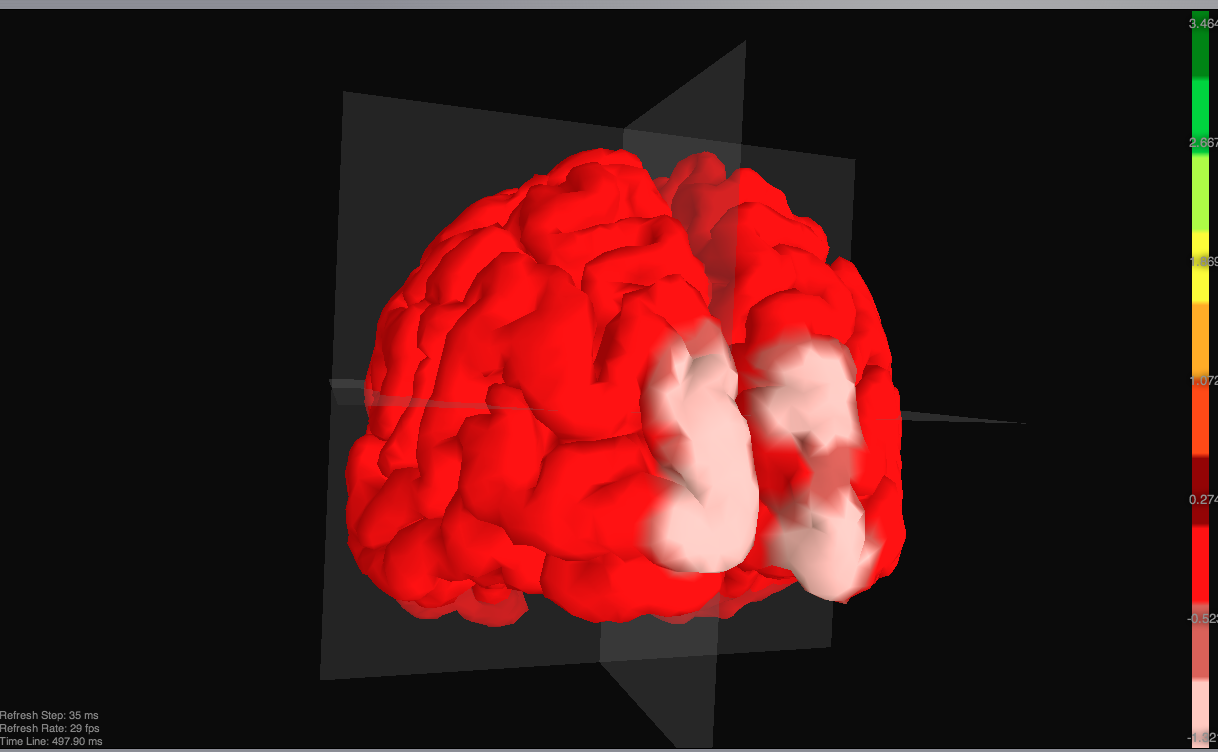
\includegraphics[width=\linewidth]{Handout_UI_HeterogenousModelAndStimulation_SurfaceStimSurfaceSim.png}%
  \caption{Surface simulation with a stimulus defined at the surface level.}%
  \label{fig:surfstim_surfsim}%
\end{marginfigure}

\begin{marginfigure}
  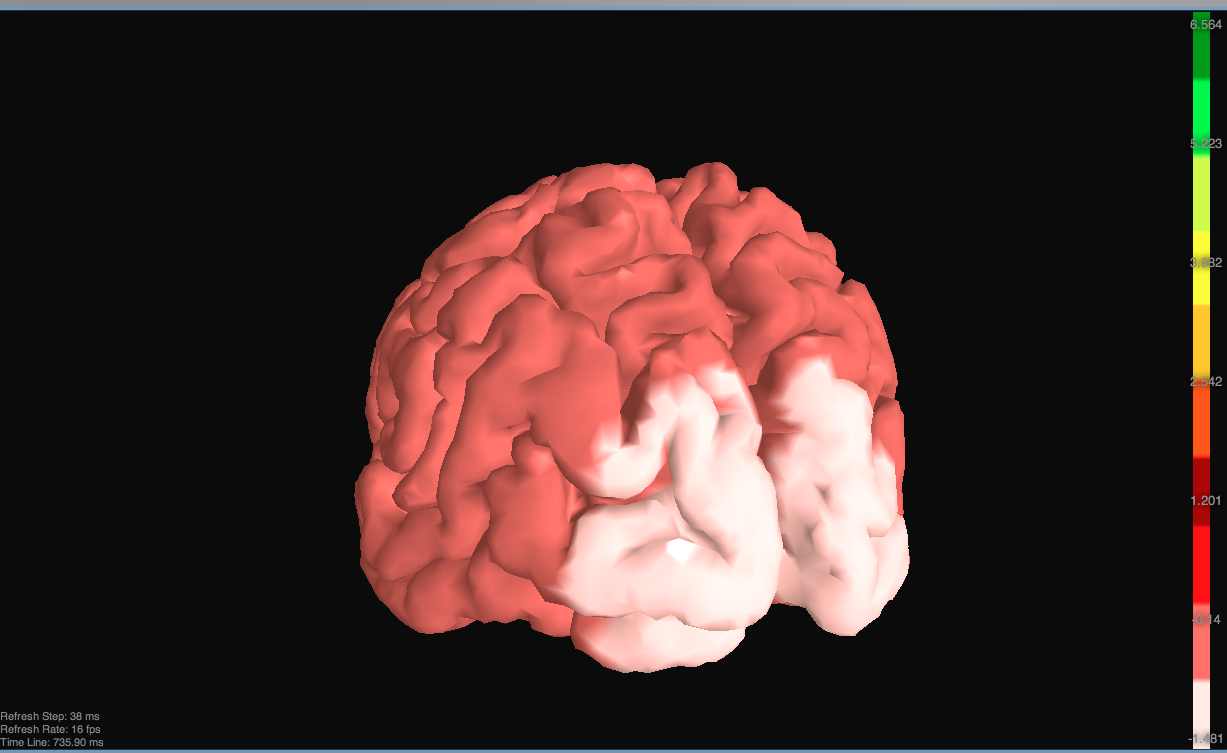
\includegraphics[width=\linewidth]{Handout_UI_HeterogenousModelAndStimulation_RegionStimSurfaceSim.png}%
  \caption{Surface simulation with a stimulus defined at the region level.}%
  \label{fig:regstim_surfsim}%
\end{marginfigure}


\subsection{Heterogeneous models}\label{sec:spatialization}

So far, we have assumed that every node either in a region or surface
simulation has the same dynamics. TVB allows for the "spatialization" of
parameters, that is, every node can have different dynamical regimes by
varying the models parameters. This feature becomes relevant when modelling
regions or patches of the brain that have different dynamics. A specific case
will be presented in the next session about modelling epilepsy in TVB.

For \underline{region simulations} the mechanism is similar as the one for creating \underline{Region
Stimulus} and for surface simulations a spatial profile determines the
variation of the parameter according to a smooth function.

\begin{figure}[h]
  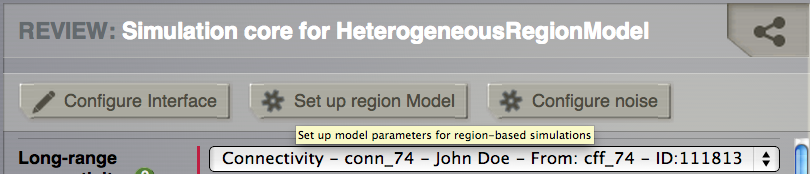
\includegraphics[width=\linewidth]{Handout_UI_HeterogenousModelAndStimulation_SetUpRegionModel.png}%
  \caption{Click on \underline{Set Up Region Model}.}%
  \label{fig:setup_regionmodel}%
\end{figure}

\begin{simulation}
\begin{enumerate}
\item For \underline{region simulations}, set up a simulation using the \underline{generic 2d oscillator} with the parameters from Table 2  found in the \textsc{Buidling Your Own Brain Network Model} handout. 
\item \item Run a simulation for \textbf{\unit[1000]{ms}}, with \underline{HeunDeterministic} and $\mathbf{dt=}$\textbf{\unit[0.1]{ms}}; use the \underline{Temporal Average} monitor with a \underline{sample period} equal to \textbf{\unit[1]{ms}}.  This is simulation \textit{HomogeneousRegionModel}.
\item Next, configure a second simulation with the same parameters as before (e.g., by coping the previous simulation). 
\item Click on \underline{Set Up Region Model} (see Fig. \ref{fig:setup_regionmodel}). We'll change the value of the model parameter \textbf{b} for a selection of nodes. This selection is already available under the name \textit{oscillatory\_nodes}. (Fig. \ref{fig:oscillatory_nodes})
\end{enumerate}
\end{simulation}

\begin{figure}[h]
  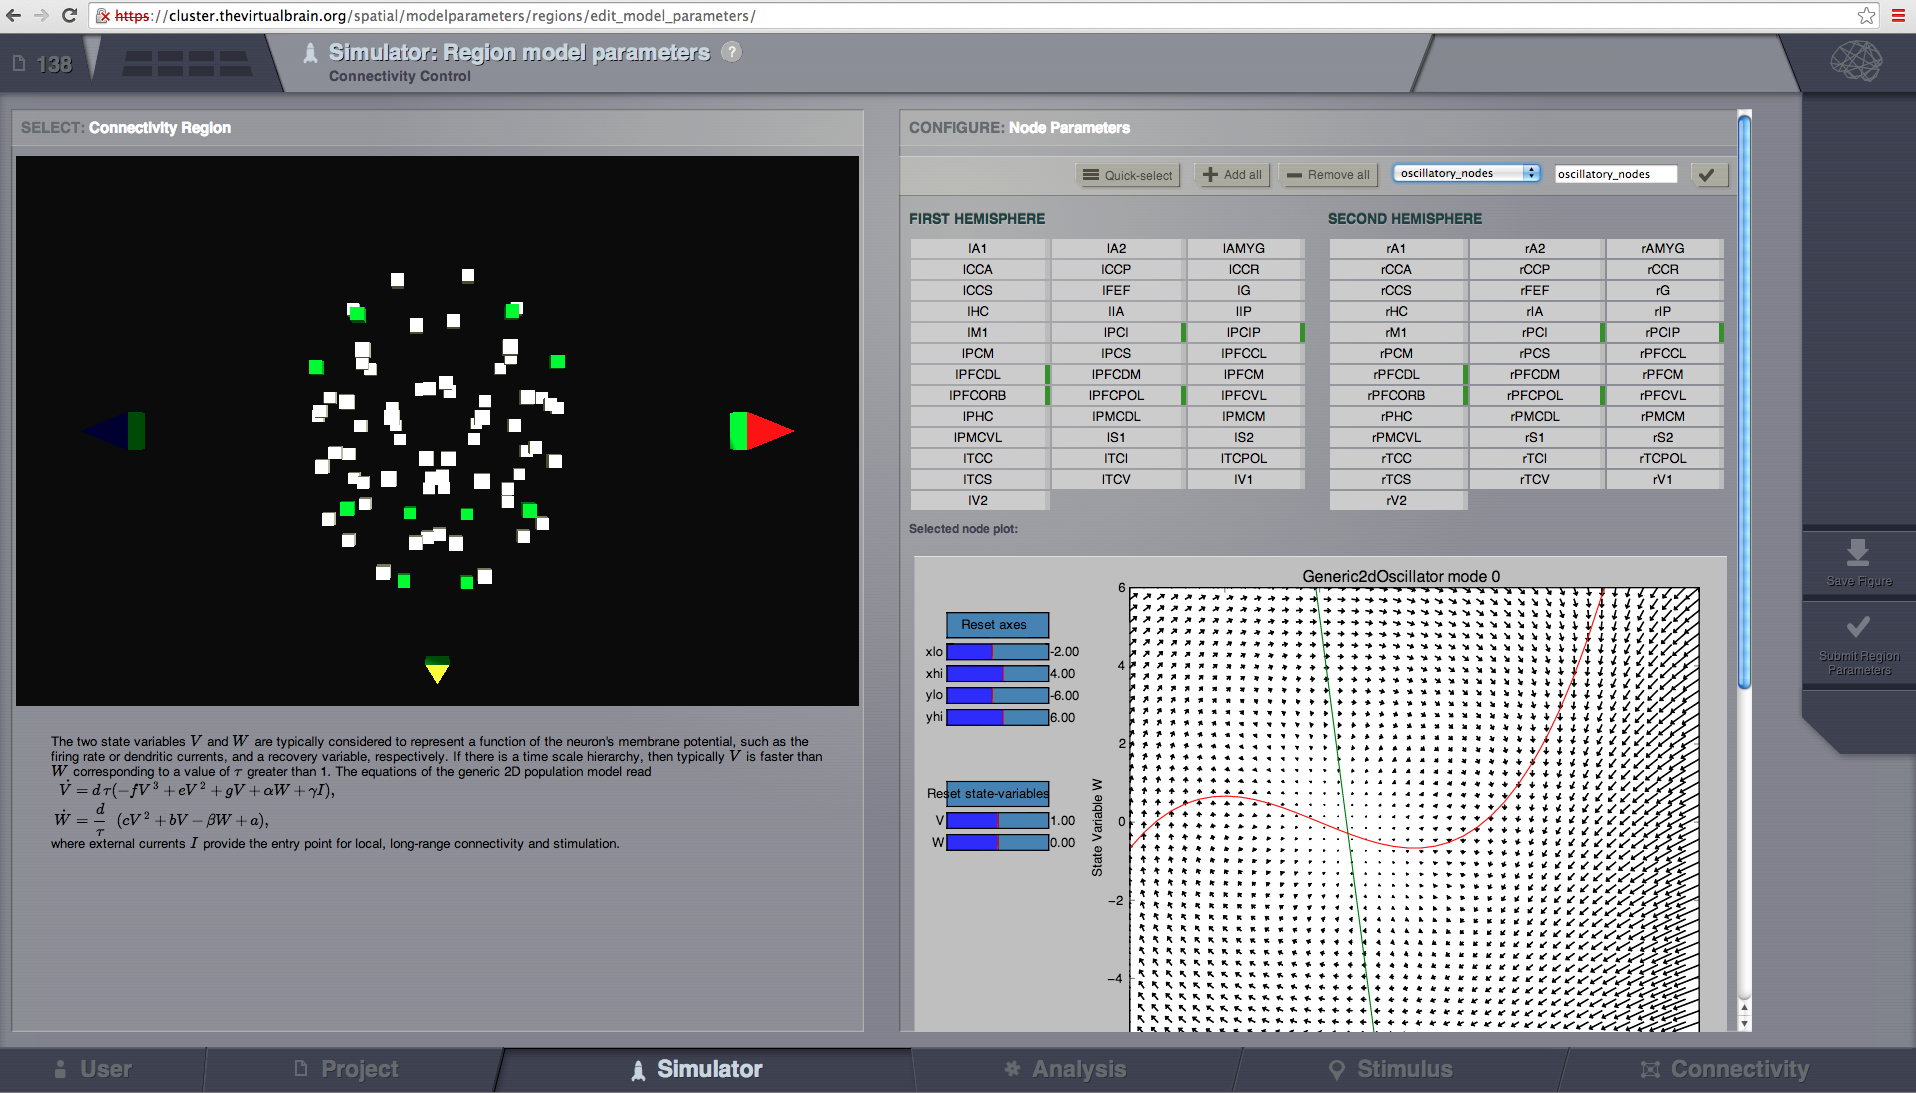
\includegraphics[width=\linewidth]{Handout_UI_HeterogenousModelAndStimulation_SpatializationSelectNodes.png}%
  \caption{Select the nodes that will have a different value.}%
  \label{fig:oscillatory_nodes}%
\end{figure}

\begin{simulation}
\begin{enumerate}
\setcounter{enumi}{4}
\item Under the \underline{Phase Plane}, change the parameter \textbf{b} to a value of approximatevely \textbf{\unit[3.7]}. Click on the \underline{pahse plane} and observe the changes. (Fig. \ref{fig:oscillatory_nodes_trajectory}).
\item Click on \textit{Submit Region Parameters}. This action will take you back to the \textsc{simulator} page. You'll see that the parameter \textbf{b} is a vector with different values for each node. 
\item This simulation corresponds to  \textit{HeterogeneousRegionModel}.
\end{enumerate}
\end{simulation}

\begin{figure}[h]
  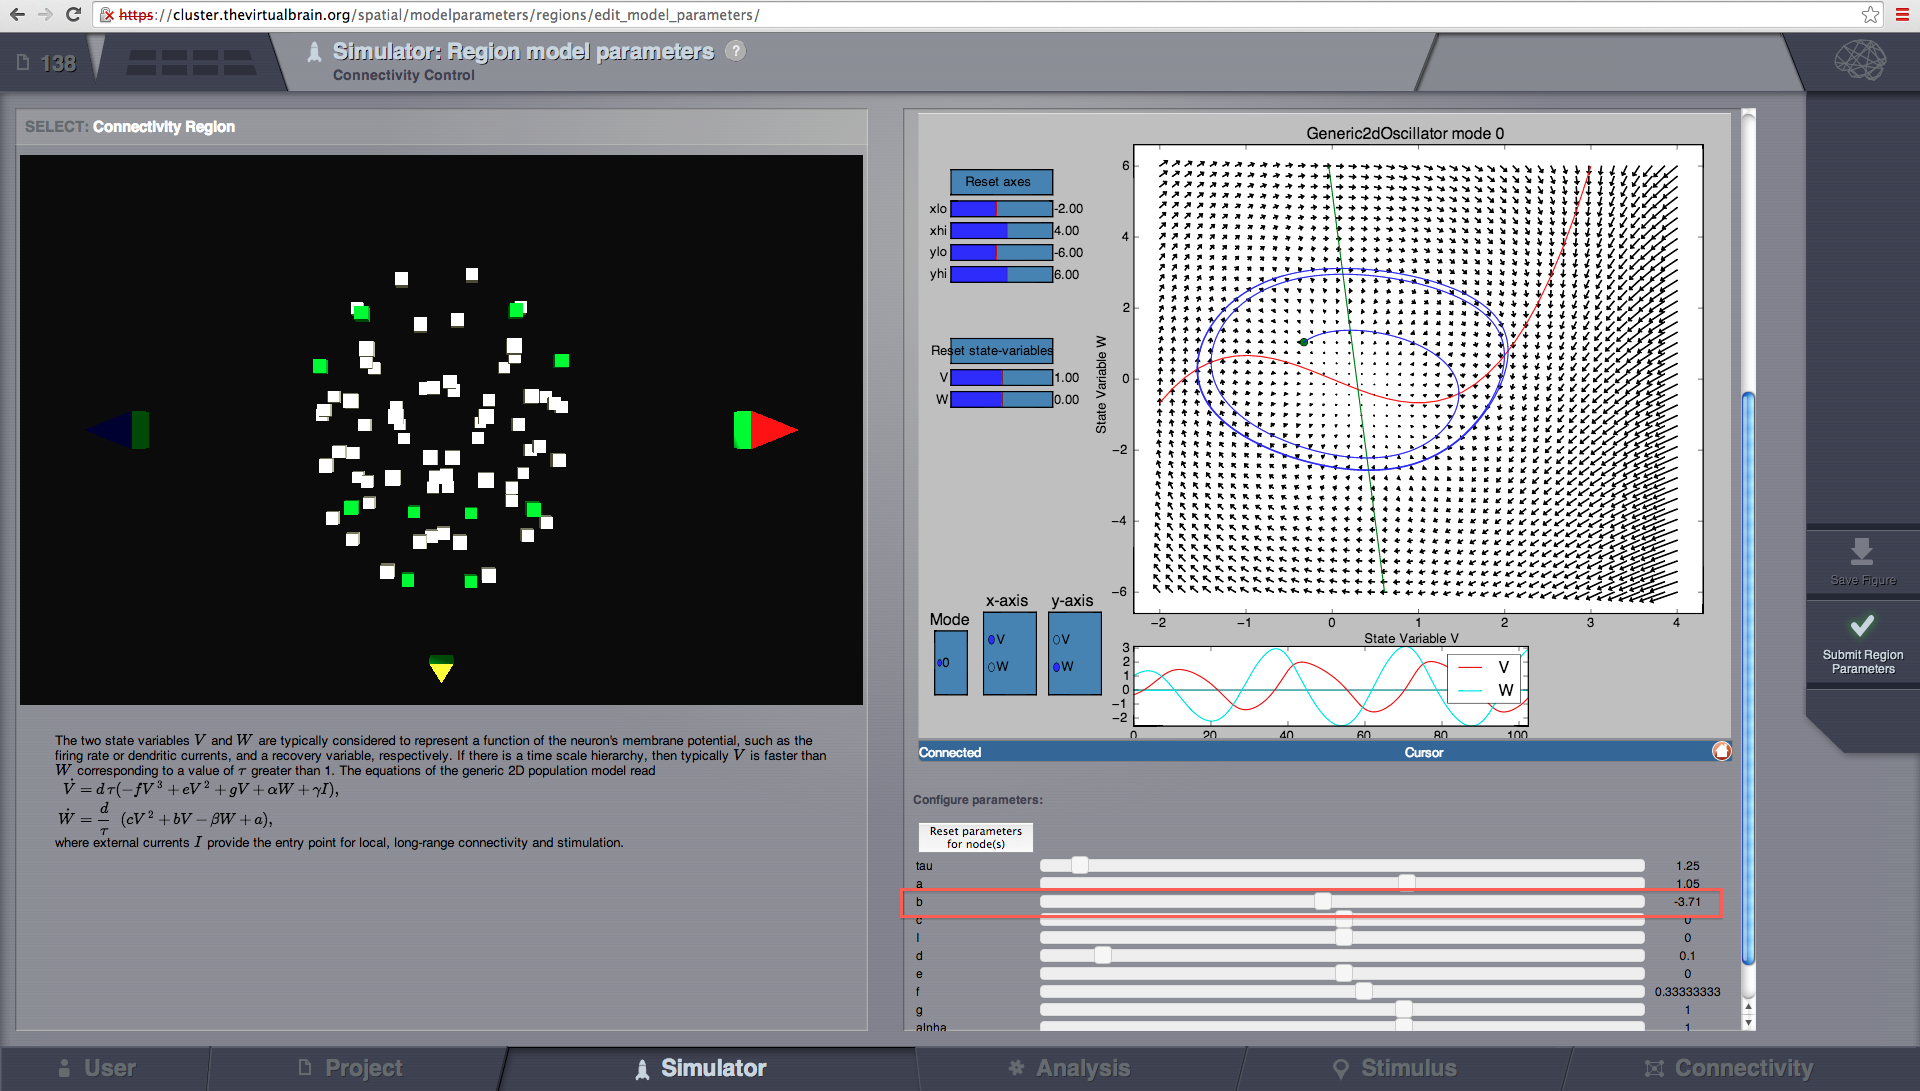
\includegraphics[width=\linewidth]{Handout_UI_HeterogenousModelAndStimulation_SpatializationChangeParameter.png}%
  \caption{Change the parameter value for the selected nodes.}%
  \label{fig:oscillatory_nodes_trajectory}%
\end{figure}



\begin{marginfigure}
  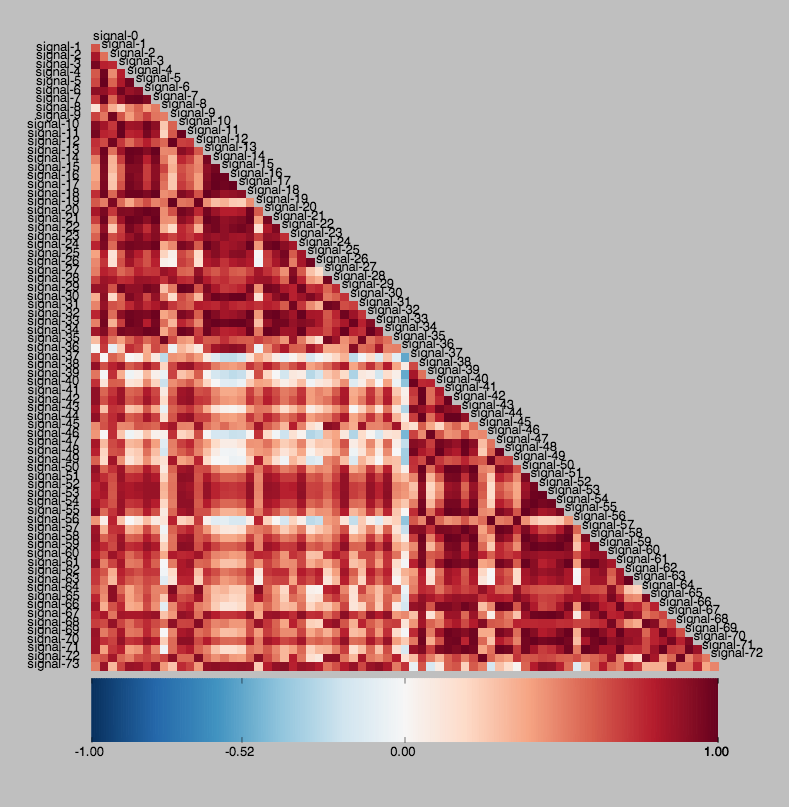
\includegraphics[width=\linewidth]{Handout_UI_HeterogenousModelAndStimulation_PearsonHomogenousSurface.png}%
  \caption{Pearson correlation coefficients computed from \textit{HomogenenousSurface
Model}.}%
  \label{fig:fc_homogeneous_surface}%
\end{marginfigure}


\begin{simulation}
\begin{enumerate}
\item For \underline{surface simulations}, copy the parameters from \textit{HomogeneousRegionModel}. Add the \underline{cortical surface}, \underline{local connectivity}. Set the \underline{local coupling strength} to \textbf{\unit[0.1]{au}}.
\item Select only the \underline{Spatial Average} monitor with a \underline{sampling period} of \textbf{\unit[1]{ms}}.
\item Run the simulation for \textbf{\unit[2000]{ms}}. The results should be those of \textit{HomogeneousSurfaceModel}. (Fig. \ref{fig:fc_homogeneous_surface}).
\item Make a copy of this simulation (e.g. \textit{HeterogenenousSurfaceModel}).
\item Click on \underline{Set Up Surface Model}.
\item Select the model parameter \textbf{b} from the drop down menu.
\item We'll use a \underline{Gaussian} function to define how this parameter will over space. The \underline{amplitude} will be \textbf{\unit[-3.0]{au}} and the width of the kernel, \underline{sigma} equal to \textbf{\unit[15][mm]}. (Fig. \ref{fig:surface_spatialization})
\item \underline{Submit the Surface Parameters}. 
\end{enumerate}
\end{simulation}

\begin{figure}[h]
  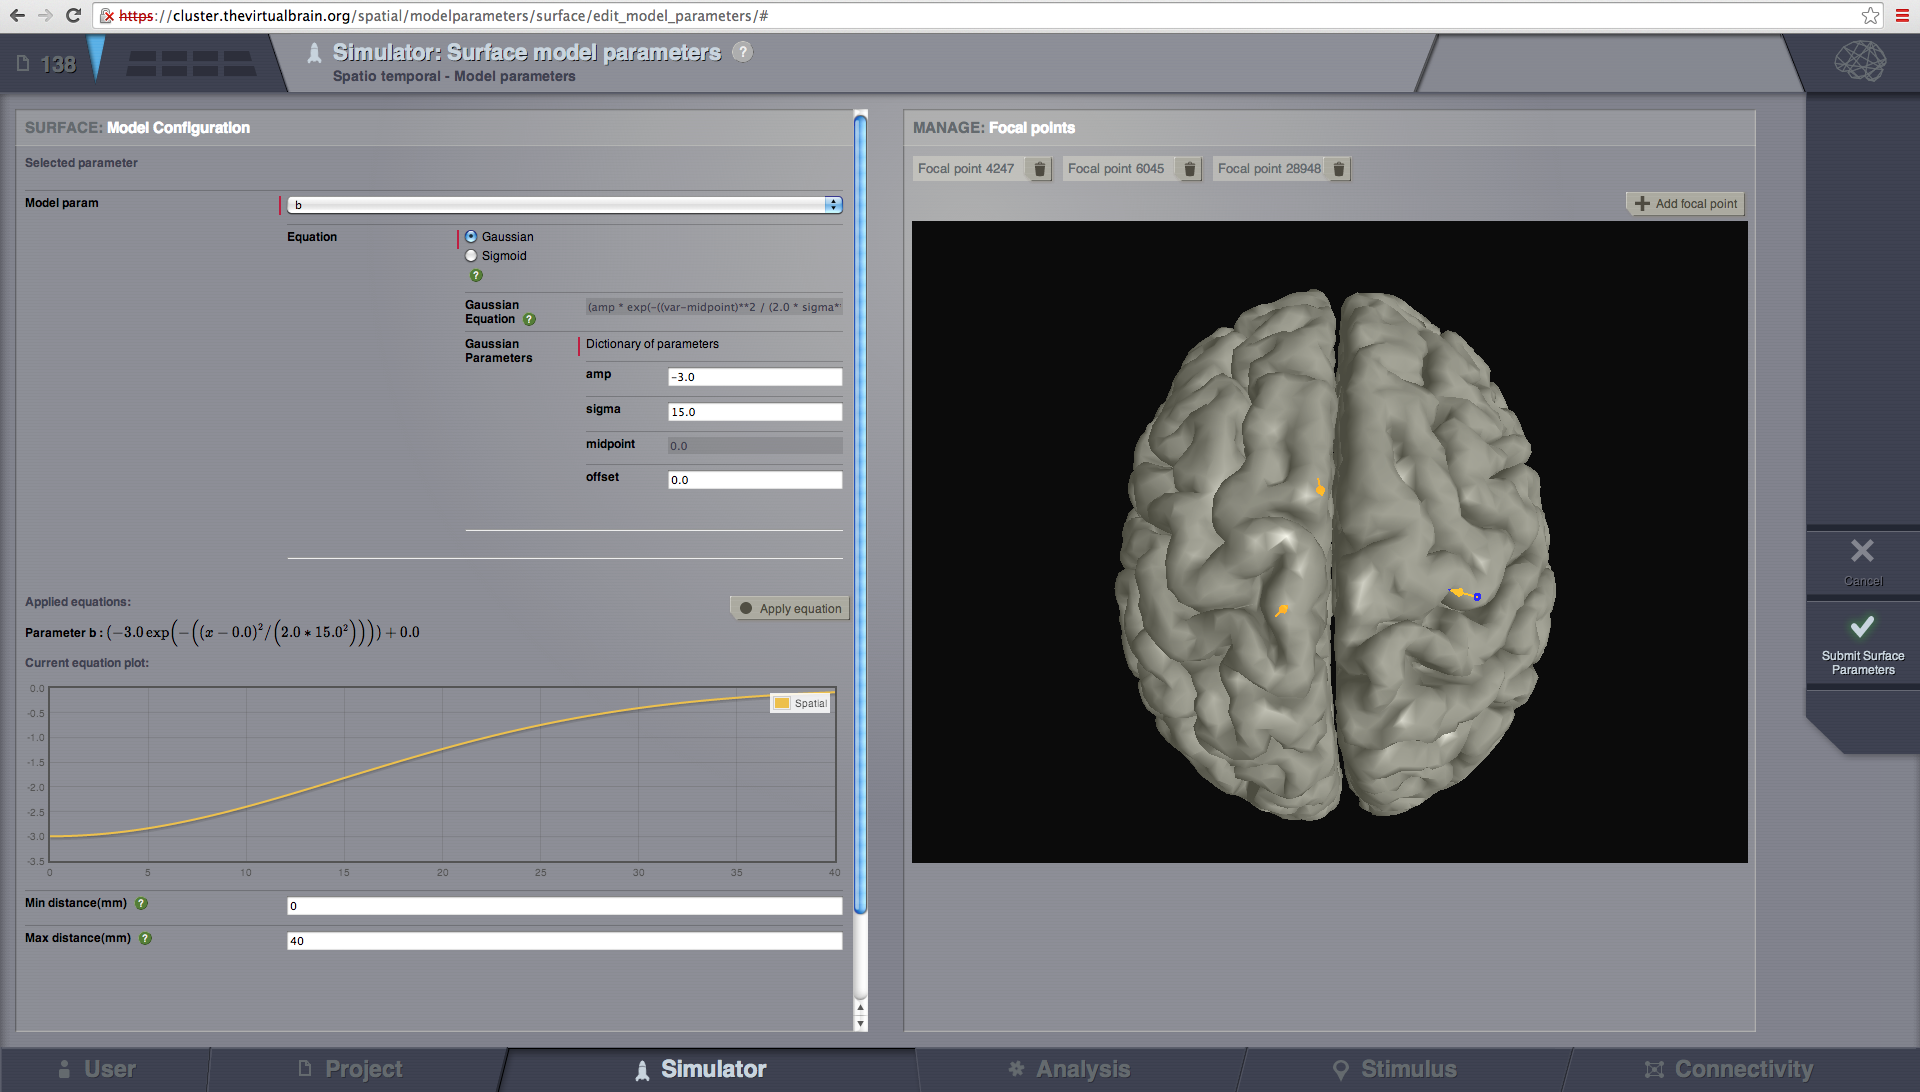
\includegraphics[width=\linewidth]{Handout_UI_HeterogenousModelAndStimulation_SurfaceSpatialization.png}%
  \caption{Describe a parameter spatial variation with a function.}%
  \label{fig:surface_spatialization}%
\end{figure}

\begin{simulation}
\begin{enumerate}[resume]
\setcounter{enumi}{8}
\item You can now launch the simulation and observe the difference with respect to the homogeneous version. (Fig. \ref{fig:fc_heterogeneous_surface}).
\end{enumerate}
\end{simulation}

\begin{marginfigure}
  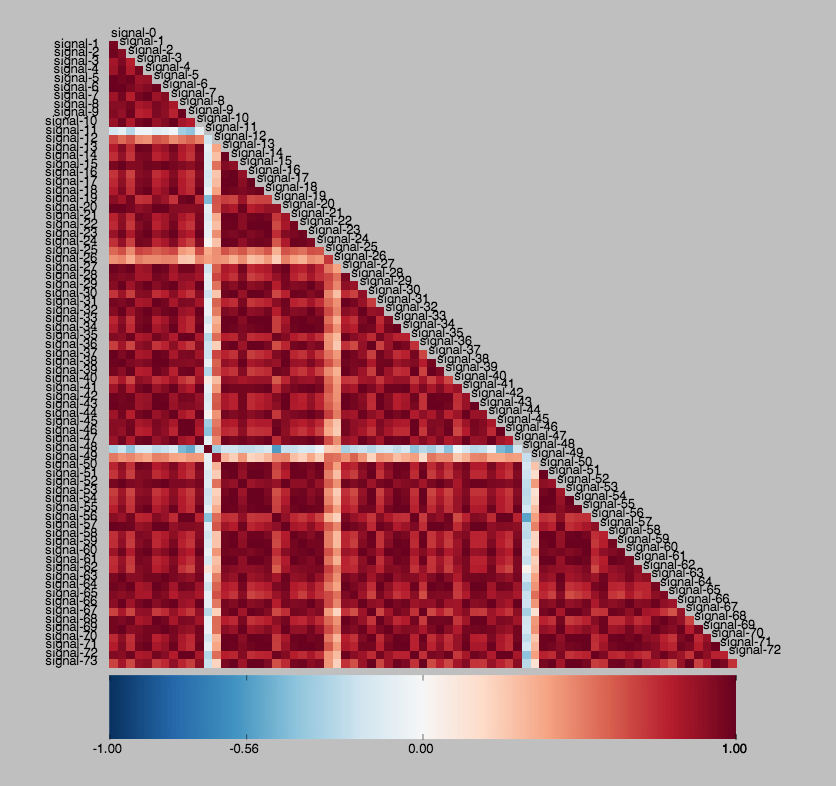
\includegraphics[width=\linewidth]{Handout_UI_HeterogenousModelAndStimulation_PearsonHeterogeneousSurface.png}%
  \caption{Pearson correlation coefficients computed from \textit{HeterogeneousSurfaceModel}.}%
  \label{fig:fc_heterogeneous_surface}%
\end{marginfigure}







\section{More Documentation}\label{sec:more-doc}
For more documentation on The Virtual Brain, please see the following articles \citep{Sanz-Leon_2013, Spiegler_2013, Woodman_2014, Jirsa_2010b}


\section{Support}\label{sec:support}

The official TVB webiste is \url{www.thevirtualbrain.org}.  
All the documentation and tutorials are hosted on \url{the-virtual-brain.github.io}.
You'll find our public \smallcaps{git} repository at \url{https://github.com/the-virtual-brain}. 
For questions and bug reports we have a users group \url{https://groups.google.com/forum/#!forum/tvb-users}

\bibliography{tvb_references}
\bibliographystyle{plainnat}

\end{document}


































































